\documentclass[11pt,dvipdfmx,a4paper]{jsarticle}

\usepackage{amsmath,amssymb}
\usepackage{bm}
\usepackage[dvipdfmx]{graphicx}
\usepackage{physics} % http://mirrors.ibiblio.org/CTAN/macros/latex/contrib/physics/physics.pdf
\usepackage{siunitx} %SI単位を楽に出力
\usepackage{mathtools} %環境の追加
% \usepackage{circuitikz} %電気回路をtex中で書く
% \usepackage{caption} %番号なしキャプションを書く
% \usepackage{cancel} %式中に斜線を入れる
% \usepackage{tensor} %テンソルの添え字を書く
% \usepackage{tikz} %図を書く
% \usepackage{ascmac} %四角い枠の中に文章を書く
% \usepackage{float} %figureで[hbp]オプションを使う
% \usepackage{hyperref}  \usepackage{pxjahyper} %ハイパーリンクをつかう
% \usepackage{tablefootnote} %表中に注釈をいれる
% \usepackage[thicklines]{cancel} %数式中の取り消し線
% \usepackage[version=4]{mhchem} %化学式の入力
\usepackage{pdfpages}
% \usepackage{wrapfig} %文章の回り込み
\usepackage[subrefformat=parens]{subcaption} %(a)図のようにすることができるやつ
\usepackage{here}
\usepackage[margin=15mm]{geometry} %余白の削除

\graphicspath{{./image/}}

\begin{document}

%出力したpdfを表紙にするとき
% \includepdf[pages=1,noautoscale=false]{cover.pdf}
% \newpage

%texで表紙を書くとき
\quad\\[35mm]
\centerline{\Huge{\textsf{第 1 回}}}
\quad\\[5mm]
\centerline{\Huge{\textsf{応 用 物 理 学 実 験}}}
\quad\\[5mm]
\begin{table}[h]
	\centering
	\begin{tabular}{| c | c |}
		\hline
		\Huge\textsf{{題目}} & \Huge{\textsf{X 線回折}} \rule[-5mm]{0mm}{15mm} \\
		\hline
	\end{tabular}
\end{table}
\quad\\[10mm]
\begin{table}[h]
	\centering
	\begin{tabular}{l l}
		\hline
		\LARGE{\textsf{氏\qquad 名}} & \LARGE{\textsf{: 西原 翔}} \rule[0mm]{0mm}{6mm} \\
		\hline
		\LARGE{\textsf{学  籍  番  号}} & \LARGE{\textsf{: 1522068}} \rule[0mm]{0mm}{6mm} \\
		\LARGE{\textsf{学部学科学年}} & \LARGE{\textsf{: 理学部第一部応用物理学科3年}}\\
		\hline
	\end{tabular}
\end{table}
\quad\\[10mm]
\centerline{\LARGE{\textsf{共同実験者:1522064 中井空弥}}}\\[2mm]
\centerline{\LARGE{\textsf{\qquad\qquad\quad\;\;1522091 宮田祟杜}}}\\[2mm]
\centerline{\LARGE{\textsf{\qquad\qquad\quad\;\;1522095 村山涼矢}}}\\[2mm]
\centerline{\LARGE{\textsf{\qquad\qquad\quad\;\;1522B02 中村洸太}}}\\[2mm]
\quad\\[10mm]
\centerline{\LARGE{\textsf{提出年月日:2024年05月02日}}}\\[2mm]
\centerline{\LARGE{\textsf{実験実施日:2024年04月19日}}}\\[2mm]
\centerline{\LARGE{\textsf{\qquad\qquad\quad\;2024年04月26日}}}
\quad\\[10mm]
\centerline{\LARGE{\textsf{東 京 理 科 大 学 理 学 部 第 1 部}}}\\[2mm]
\centerline{\LARGE{\textsf{応 用 物 理 学 教 室}}}

\thispagestyle{empty}
\clearpage
\addtocounter{page}{-1}
\newpage

% \twocolumn
\section{目的}
金属やイオン結晶といった固体は一つ一つの原子がある一定の規則性をもって配置している。
十分細いスリットにコヒーレント光を当てると、
光はスリットで回折を起こしスクリーンにパターンが浮かび上がる。
このパターンから目には見えないスリット幅が求めることができるように、
結晶に光を当てるとそれをなす原子間距離やその構造を回折パターンから求めることができる。
特に光源に X 線、ターゲット試料を粉末にしたものを粉末 X 線回折測定法 (X-Ray Diffraction, XDR)
と呼ばれる。この実験では立方晶系の材料 Cu, Si, Fe の単体粉末と、NaCl, KCl, CsCl の
粉末試料にCu の特性 X 線を入射したときの回折パターンから、その試料の格子定数を求めた。
またこの測定において Fe と NaCl, KCl, CsCl に X 線を当てたときの振る舞いについて考察した。

\section{原理}
\subsection{回折の一般論}
回折の一般論を確認する。
光源から出た光や、回折して検出器に入る回折光は本来は球面波である。
しかし、ターゲット材料との距離が十分離れているときには平面波のように扱うことができる。

光源から出た光が点 P で弾性散乱して点 B の検出器に到達するという過程を考える。(図\ref{ibach_fig3-1})
\begin{figure}[H]
	\centering
	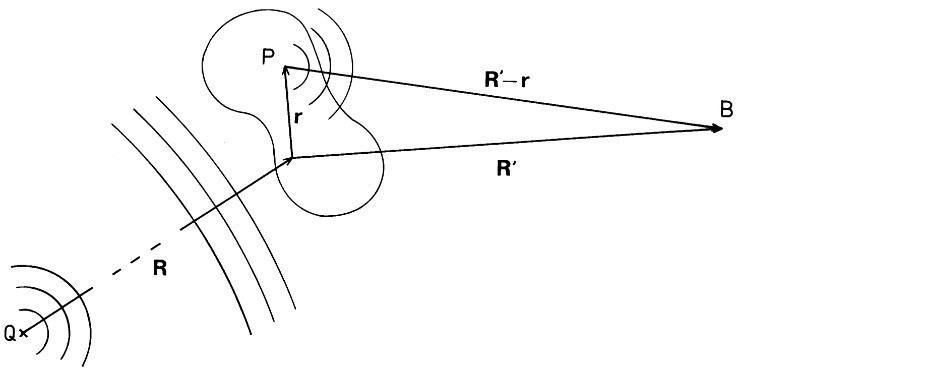
\includegraphics[width = \columnwidth]{/fig/ibach_3-1.png}
	\caption{散乱による回折の模式図。\cite{ibach-luth}}
	\label{ibach_fig3-1}
\end{figure}
点 P における入射光の状態は弾性散乱であるため位相の時間部分を略して
\begin{align}
	A_P(r) = A_0e^{ik_0\cdot(R+r)}
\end{align}
と書ける。ここで\(\rho(r)\)は散乱密度。

古典的には散乱光は
入射波の電磁場が結晶中の荷電粒子を振動させたことによる加速電荷が放射する電磁波である。
加速運動するときに質量\(m\)の電荷のが放出するエネルギーは Lamor の公式より
\begin{align}
	\dv{W}{t} = \frac{q^2}{6\pi\varepsilon_0c^3}\abs{\ddot{r}}^2
\end{align}
となる。また電荷の従う運動方程式は
\begin{align}
	m\ddot{r} = qE^{i(k\cdot r -\omega t)}
\end{align}
より
\begin{align}
	\dv{W}{t} \propto \frac{1}{m^2}
\end{align}
となる。原子核より電子の方が軽いので放射するエネルギーは電子からによるものがほとんどだとわかる。
これより光の回折は結晶中の電子がするものと言える。
散乱密度はこのようにして電子の密度であることが示された。

散乱により振幅と位相が変わるので点 B での散乱光の振幅は
\begin{align}
	A_B(r) &= A_P \rho(r) \frac{e^{ik\cdot(R'-r)}}{R'}\\
	&=\frac{A_0}{R'}e^{i(k_0 \cdot R+ k \cdot R')}\rho(r)e^{i(k_0-k)\cdot r}
\end{align}
となる。ターゲット材料全体で積分すると検出器が実際に検出する振幅になるので積分すると
\begin{align}
	A_B =\frac{A_0}{R'}e^{i(k_0 \cdot R+ k \cdot R')}\int \rho(r) e^{i(k_0-k)\cdot r} dr.
\end{align}
このうち積分の部分を原子散乱因子\(f\)と呼ぶ。
結晶材料を考えるとき、原子散乱因子は結晶の周期性からくる散乱条件と、単位格子内の原子の配置による散乱条件がある。
前者は Laue 条件(等価なものとして Bragg の条件)、後者は結晶構造因子と呼ばれる。

これが見えやすい形に原子散乱因子の積分を書き換える。
積分の引数の \(r\) を格子の位置を表す \(R\), 格子中の j番目の原子の位置を表す \(r_j\), そして
格子中の j 番目の原子の周りの散乱密度を\(\rho_j\)と表すと、
\begin{align}
	f&=\sum_R \sum_{j} \int\rho(r-R-r_j)e^{i(k_0-k)\cdot r} dr\\
	&=\sum_R e^{-iK\cdot R}\sum_j e^{-iK\cdot r_j} \int \rho_j(r-R-r_j) e^{-iK\cdot(r-R-r_j)}dr\label{factor_1}
\end{align}
となる。ここで入射波と散乱波の波数ベクトルの差を
\begin{align}
	K = k -k_0
\end{align}
とした。

\subsection{Laue の回折条件}
(\ref{factor_1})式の \(R\) についての総和について考える。
\(R = n_a a + n_b b + n_c c\) というように格子ベクトルで展開して、
a 軸、b 軸、c 軸の格子数を\(N_a,\,N_b,\,N_c\) とすると総和は
\begin{align}
	G(K) &:= \sum_R e^{-iK\cdot R}\sum_j e^{-iK\cdot r_j}\\
	&= \sum_{n_a=1}^{N_a} e^{-in_aK\cdot a} + \sum_{n_b=1}^{N_b} e^{-in_bK\cdot b} + \sum_{n_c=1}^{N_c} e^{-in_cK\cdot a}\\
	&=\frac{e^{-iK\cdot a} (1-e^{-iN_a K\cdot a})}{1-e^{-iK\cdot a}}\,
	\frac{e^{-iK\cdot b} (1-e^{-iN_b K\cdot b})}{1-e^{-iK\cdot b}}\,
	\frac{e^{-iK\cdot c} (1-e^{-iN_c K\cdot c})}{1-e^{-iK\cdot c}} .
\end{align}
これよりこの部分による回折強度は
\begin{align}
	\abs{G(K)}^2 &= \dfrac{\sin^2(N_a K\cdot a/2)}{\sin^2(K\cdot a/2)}
	\dfrac{\sin^2(N_b K\cdot b/2)}{\sin^2(K\cdot b/2)}
	\dfrac{\sin^2(N_c K\cdot c/2)}{\sin^2(K\cdot c/2)} .
\end{align}
これより \(K\) が
\begin{align}
	K\cdot a = 2\pi h, \qquad K\cdot b =2\pi k, \qquad K\cdot c =2\pi l
\end{align}
を満たすとき、つまり 波数ベクトルの変化が逆格子ベクトルと等しいとき
\begin{align}
	K = G_{hkl}
\end{align}
において回折強度を持つ。これを Laue の条件という。
% Ewalt 球らへんでアンブレラ効果をやりたい

\subsection{Bragg の回折条件}
 Laue の条件と等価な条件式を導く。
逆格子ベクトル \(G_{hkl}\) は格子面 (hkl) の法線ベクトル [hkl] になっている。
そのため面間隔\(d_{hkl}\)は法線ベクトルと基本格子ベクトルとの内積を考えることによって求まる。
今回は立方晶を扱うので a 軸の基本格子ベクトルを \(a\), 格子定数を\(a_0\) として
\begin{align}
	d_{hkl} &= \frac{a}{h} \cdot \frac{G_{hkl}}{\abs{G_{hkl}}}\\
	&= \frac{2\pi}{\abs{G_{hkl}}} \label{eq:d-G}\\
	&= \frac{2\pi a_0}{\sqrt{h^2+k^2+l^2}}
\end{align}
となる。
\(k\) と \(k_0\) のなす角は散乱角\(\Theta\)を用いて表すと \(2\Theta\) であり、これを使って \(K\) の大きさを表すと
\begin{align}
	\abs{K} = 2k_0\sin\Theta = \frac{4\pi\sin\Theta}{\lambda}
\end{align}
となる。Laue の条件の両辺のベクトルの大きさを取ってみると
\begin{align}
	\frac{4\pi\sin\Theta}{\lambda} &= \frac{2\pi}{d_{hkl}}\\
	2d_{hkl} \sin\Theta &= \lambda
\end{align}
これが Bragg の条件である。
また散乱角 \(\Theta\) を測定して格子定数 \(a\) と面指数 (hkl) を求めるのに面間隔 \(d_{hkl}\) を Bragg の条件から消去した式
\begin{align}
	\lambda \sqrt{h^2+k^2+l^2}  = 2a \sin\Theta \label{eq:bragg}
\end{align}
も使う。

\subsection{結晶構造因子}
(\ref{factor_1})式の \(j\) についての総和を考える。
Laue の条件を当てはめ、積分の引数を変換すると
\begin{align}
	F_{hkl} := \sum_j e^{-iG_{hkl}\cdot r_j} \int \rho_j(r) e^{-iG_{hkl}\cdot r_j}dr .
\end{align}
積分の部分を
\begin{align}
	f_j :=\int \rho_j(r) e^{-iG_{hkl}\cdot r_j}dr
\end{align}
とする。
\(G_{hkl}\) を逆格子ベクトルベクトルで書いたものを入れると
\begin{align}
	F_{hkl} = \sum_j f_j e^{-2\pi i (hx + ky + lz)}
\end{align}
というようになる。
このとき、結晶構造によっては\(F_{hkl}\) の値が 0 となることがある。

積分の中身\(f_j\)を評価する。電子密度 \(\rho\) を原子の周りに関して球対称だとみなすと
\begin{align}
	f_j &=\int \rho_j(r) e^{-iG_{hkl}\cdot r_j}dr\\
	&= \rho_j(r) e^{-iG_{hkl} r_j \cos\theta}r^2\sin\theta dr\\
	&= 4\pi \int \rho_j(r) r^2 \frac{\sin(Gr)}{Gr}dr\\
\end{align}
\(k\) と \(k_0\) のなす角は散乱角 \(2\Theta\) であり、これを使って表すと
\begin{align}
	G = K = 2k_0\sin\Theta = \frac{4\pi\sin\Theta}{\lambda}
\end{align}
なので
\begin{align}
	f_j  = 4\pi \int \rho(r) r^2 \frac{\sin(4\pi r\sin(\Theta \lambda))}{4\pi r(\sin\Theta/\lambda)} dr
\end{align}
となる。
これをプロットすると図\ref{graph1}となる。
\begin{figure}[H]
	\centering
	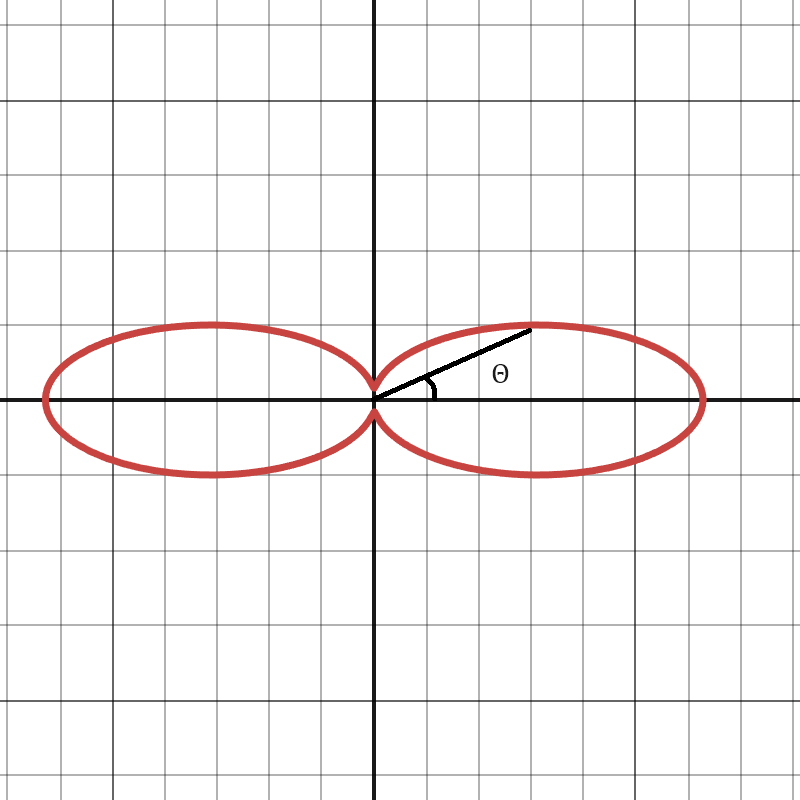
\includegraphics[width =0.5\columnwidth]{/graph/graph1.png}
	\caption{原子散乱因子。偏角に対する強度をプロットした。}
	\label{graph1}
\end{figure}
これより回折強度は\(\Theta = 0\) で最大で \(\Theta = \pi/2\) で最も弱くなる。
% https://www.desmos.com/calculator/i8apmkd23r 1s 電子でやった時の強度

\subsection{X 線源}
今回の実験で使う X 線源はタングステンフィラメントを加熱し発生した熱電子を Cu にあてて、
光電効果により発生させる。
この際、銅原子内の電子が様々な準位に励起され、励起により空いた準位に電子が遷移する際に光子(X 線)を放つ。
特に
2p 軌道から励起より空いた 1s 軌道に遷移するとき発生する X 線は K\(\alpha\) 線、
3p 軌道から励起より空いた 1s 軌道に遷移するとき発生する X 線は K\(\alpha\) 線と呼ばれる。
さらに微細構造によりK\(\alpha\)は二つに分裂しておりそれぞれを
K\(\alpha_1\) 線、K\(\alpha_2\) 線と呼ばれる。

K\(\alpha_1\) 線、K\(\alpha_2\) 線、K\(\beta\) 線の波長はそれぞれ
\begin{align}
	\lambda_{\alpha1} = 1.542 \text{\AA}\\
	\lambda_{\alpha2} = 1.540 \text{\AA}\\
	\lambda_{\beta} = 1.392 \text{\AA}\\
\end{align}
というように近い値をもつ。\cite{rikanenpyo}
これらは無視できない強度を持ち X 線の回折パターンに影響与えるためうまく取り除く必要がある。

Ni の 1s 軌道電子が空軌道へ遷移するのに必要なエネルギーの最低値が 8332.8 eV であるつまり、
Ni が吸収する波長のうち最も長いものは \(\lambda = 1.488\) \AA である。
これを利用して X 線のディテクターの前に Ni のフィルターをセットすることで K\(\beta\) 線のピークをなくすことができる。

K\(\alpha_2\) 線は波長が近いためこれによるピークが見えるものと見えないものがある。
これは測定装置に付属する解析ソフトにより除去する。

\subsection{粉末 X 線回折}
単体のターゲット試料に X 線を当てたとき、X 線が回折するのは特定の一つの面だけである。
そのため試料を回転させる等の工夫が必要となる。

万遍なく各結晶面からの回折を見るのに Debye と Scherrer はターゲット試料を粉末にした。
各粉末は小さな結晶となっていて、各結晶は向いている面がランダムになっているため回折角を調整するだけで様々な面からの散乱をみることができる。


\subsection{Nelson-Riley の式による格子定数の外挿}
(\ref{eq:bragg})式による格子定数決定をすると、実験系の系統誤差によりずれてしまう。
例えば Ewalt 球の曲面の一部を切り取ってピークにすることによるアンブレラ効果、
X 線の偏光によるずれ、ターゲット試料の回転ステージの偏心によるもの、
X 線のフォーカスによるずれ、
などがある。この系統誤差は回折角 \(\Theta = \pi/2\) のときに最小となるが、
図\ref{graph1} で見たようにこのときの回折強度は弱い。
\(\Theta = \pi/2\) の値を外挿して格子定数を求めるのに同時期に Nelson, Riley のグループと
Taylor, Sinclair のグループによって外挿する式が出された。\cite{Nelson_1945}\cite{Taylor_1945}
その式は
\begin{align}
	a(\Theta) = k\qty(\frac{\cos^2\Theta}{\sin\Theta}+\frac{\cos^2\Theta}{\Theta}) + a \label{eq:nelson-riley}
\end{align}
である。ここで \(k\) はある定数、\(a(\pi/2)=a\)の値が求める格子定数である。
Nelson, Riley のグループの論文では外挿するを比較し、最もよくできている関数として紹介している。
そのため経験的にうまくいく関数として言われるが、
Taylor, Sinclair のグループの論文では各系統誤差をモデル化し、ある系統誤差に対するものの議論でこの式を出している。
% \footnote{ちゃんと読めてないですがいいこと言ってます。}
このレポートでは(\ref{eq:bragg})式による格子定数と(\ref{eq:nelson-riley})式による格子定数の両方を求める。


\section{実験}
この実験ではリガクの MiniFlex600 を用いて、
Cu, Si, Fe の単体粉末と、NaCl, KCl, CsCl の粉末の X 線回折パターンを測定した。
その際、Ni フィルターによる K\(\beta\)線 の除去の程度を調べるため、
Cu の X 線の回折パターンはフィルターが無いときとある時の両方を測定した。
測定データはピークの位置や回折強度に大きな影響を与えない程度のバックグラウンド除去や
K\(\alpha_2\) 線によるピークを除去をした。

\section{結果}
Niフィルターの有無による Cu の X 線回折パターンは図\ref{Cu_XRD}のようになった。
Si, Fe の単体粉末と、NaCl, KCl, CsCl の粉末の X 線回折パターンは
それぞれ図\ref{Si_XRD}, 図\ref{Fe_XRD}, 図\ref{NaCl_XRD}, 図\ref{KCl_XRD}, 図\ref{CsCl_XRD} のようになった。
またこの回折ピークと結晶構造因子による消滅則を考慮しながら格子定数を求めると表\ref{table:result}のようになった。
算出法は Bragg の式 (\ref{eq:bragg})式と Nelson-Riley 関数 (\ref{eq:nelson-riley}) に測定値を入れて求めた。
\begin{table}[H]
	\centering
	\caption{X 線回折による格子定数の測定結果(単位:\AA)} \label{table:result}
	\begin{tabular}[pos]{lcccccc}
		\hline \hline
		算出法 & Cu & Si & Fe & NaCl & KCl & CsCl \\
		\hline
		Bragg の式 & 3.6219 & 5.4414 & 2.8723 & 5.6441 & 6.2898 & 4.1207 \\
		Nelson-Riley 関数 & 3.6184 & 5.4354 & 2.8688 & 5.6433 & 6.2979 & 4.1259\\
		\hline \hline
	\end{tabular}
\end{table}
\begin{figure}[H]
	\centering
	\begin{minipage}[t]{0.48\columnwidth}
		\centering
		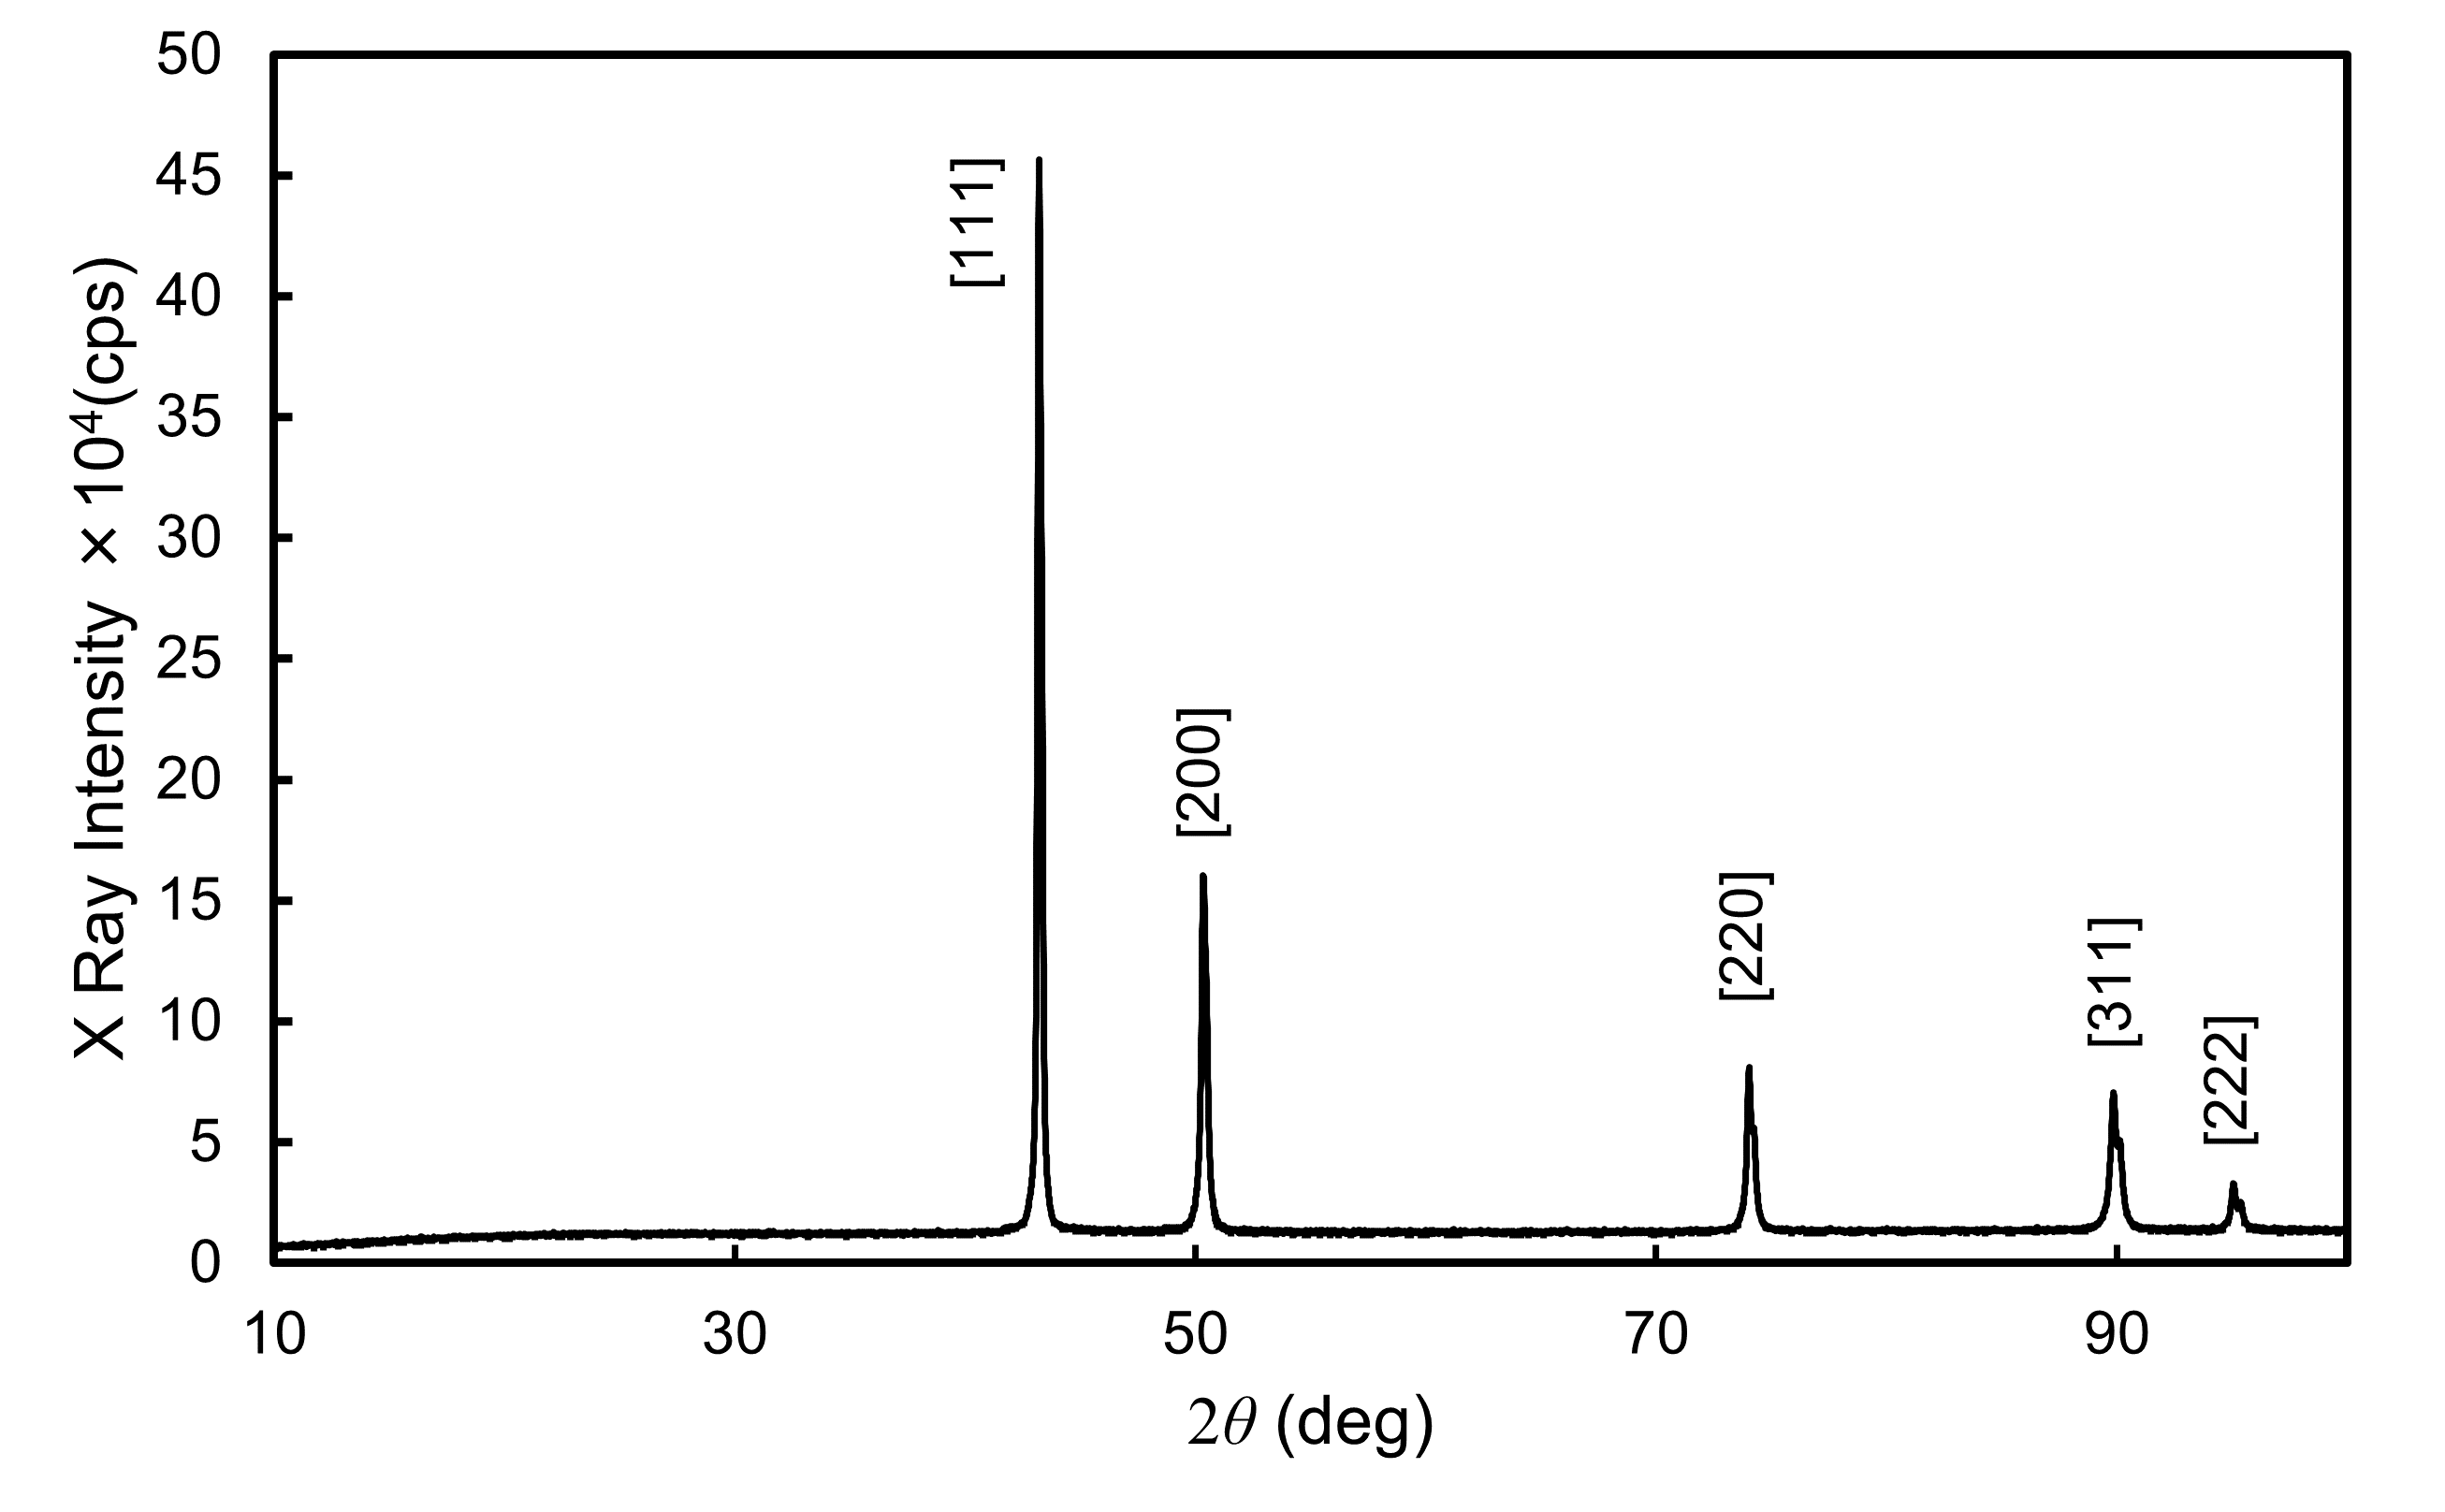
\includegraphics[width=\columnwidth]{/graph/Cu.png}
		\subcaption{Ni フィルター有}
	\end{minipage}
	\hfil
	\begin{minipage}[t]{0.48\columnwidth}
		\centering
		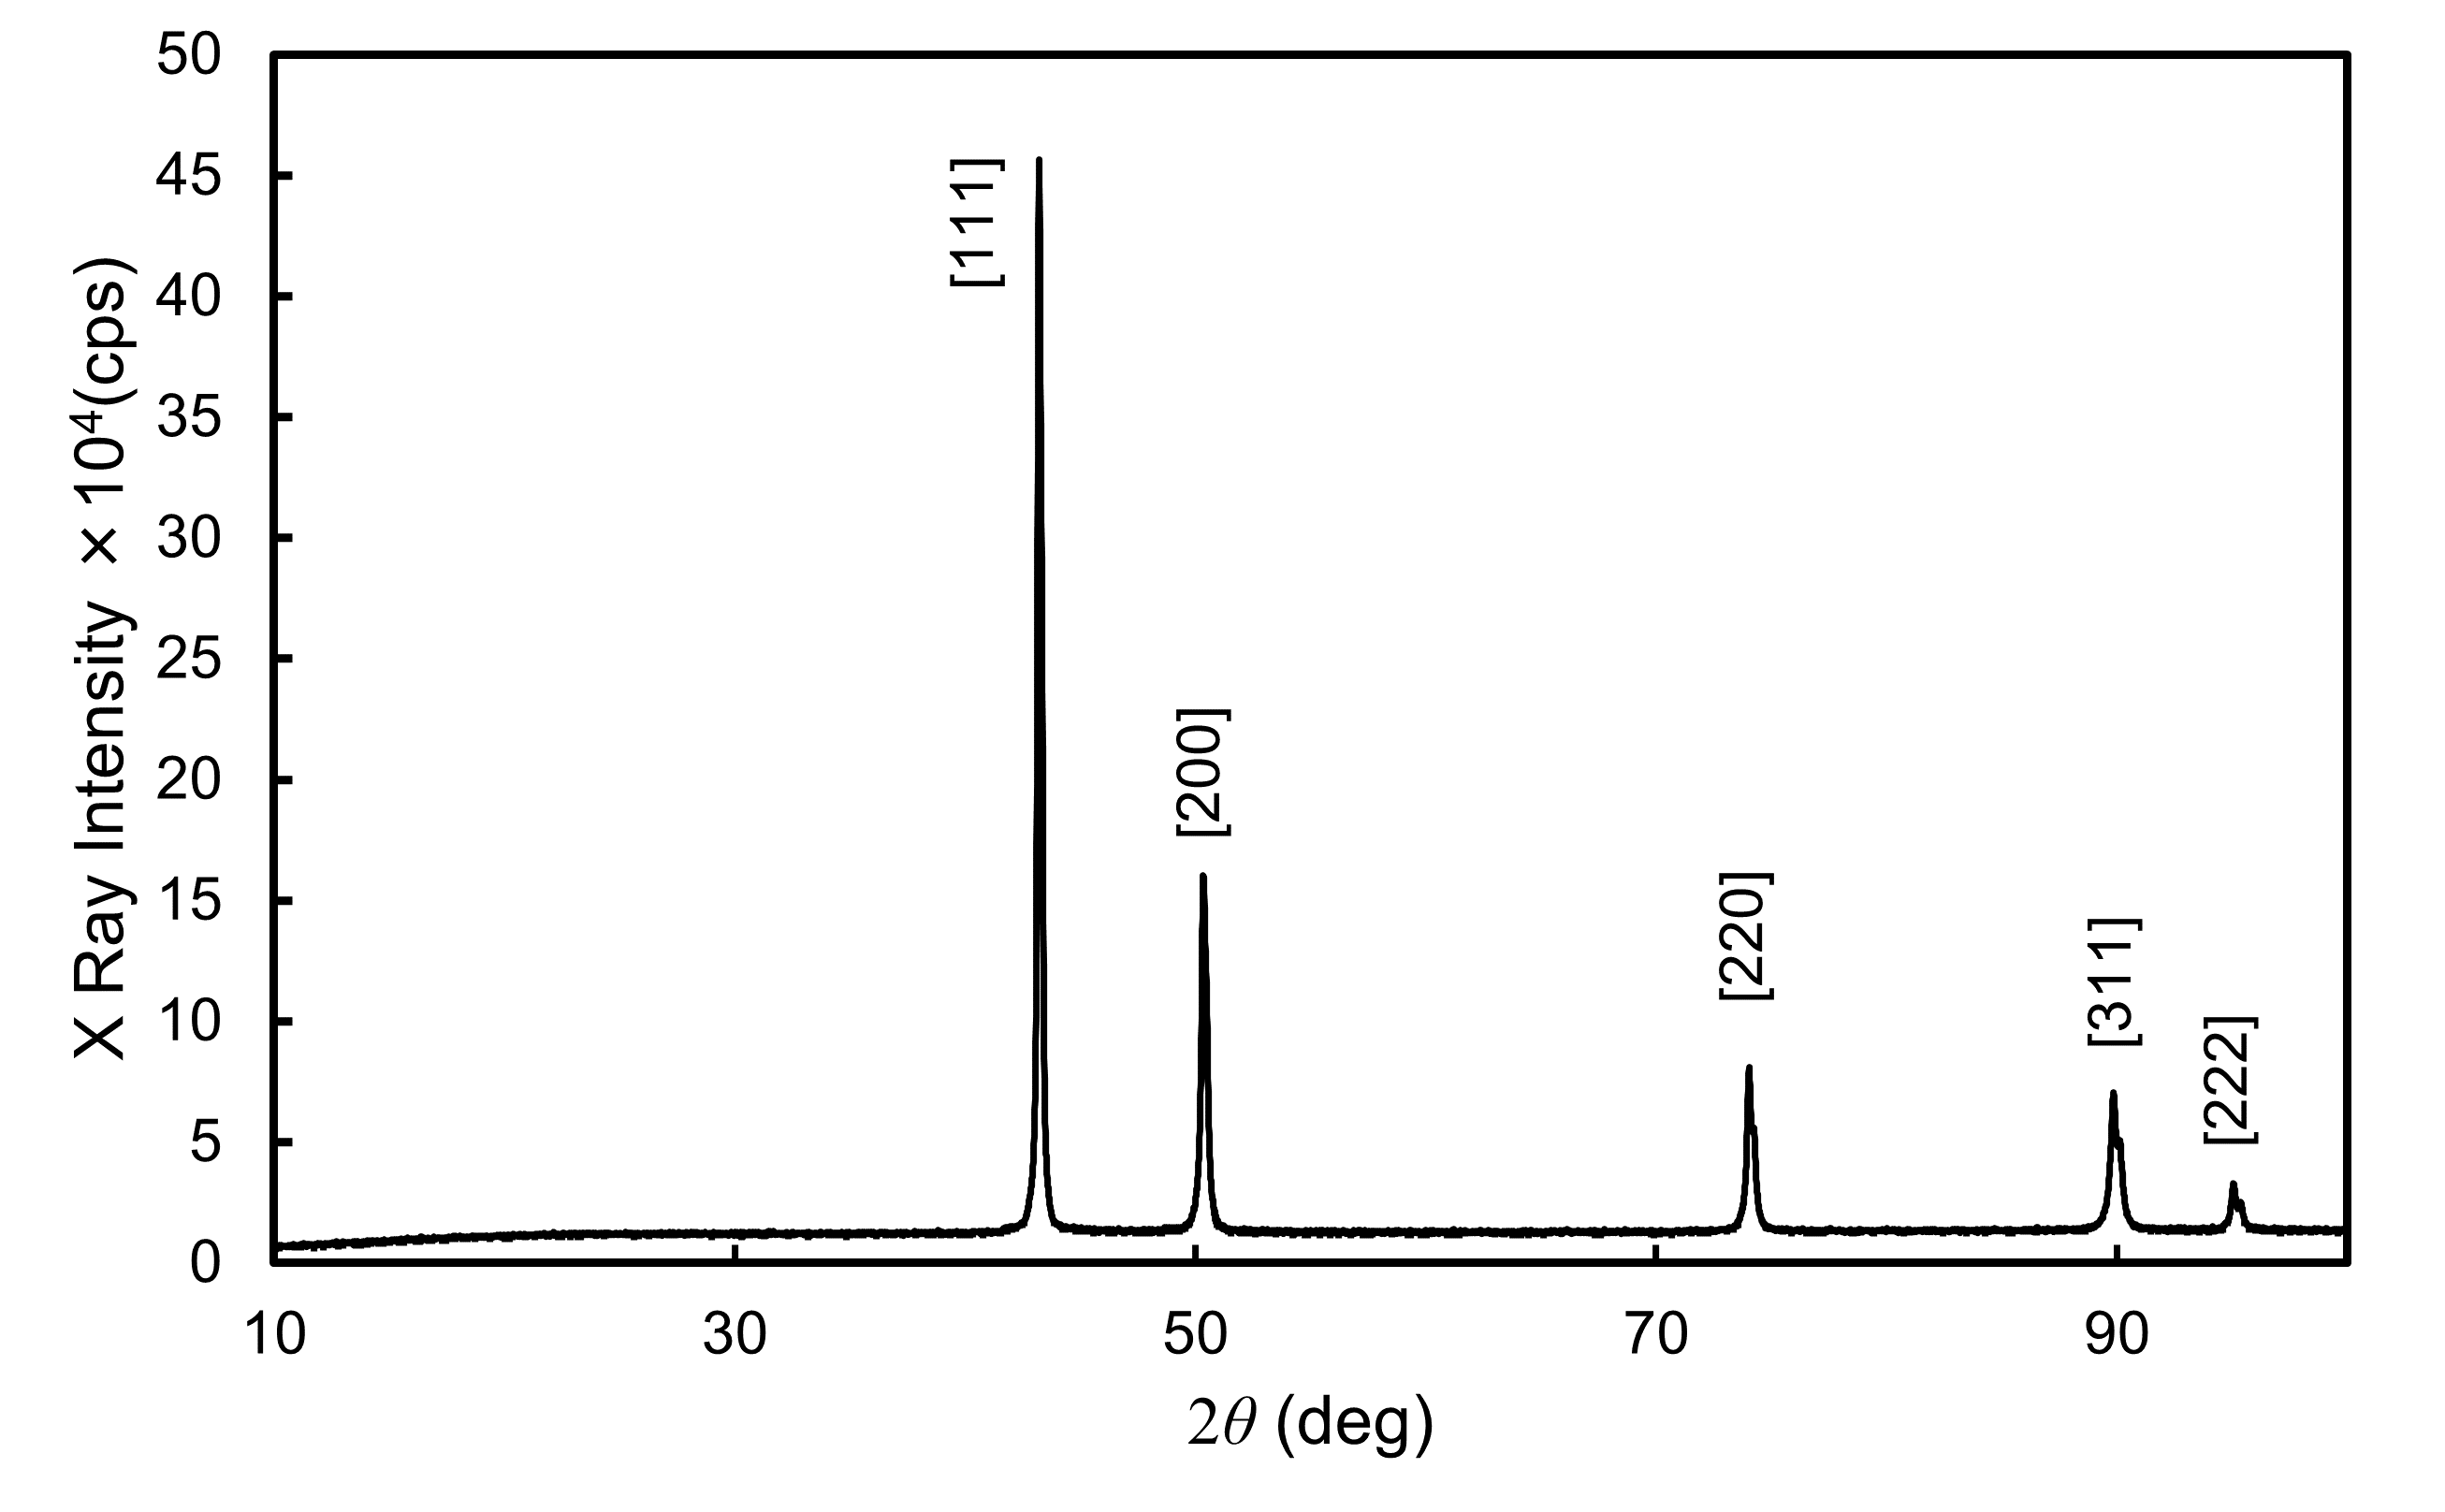
\includegraphics[width=\columnwidth]{/graph/Cu.png}
		\subcaption{Ni フィルター無}
	\end{minipage}
	\caption{Cu 単体粉末の X 線回折強度}
	\label{Cu_XRD}
\end{figure}
\begin{figure}[H]
	\centering
	\begin{minipage}[t]{0.48\columnwidth}
		\centering
		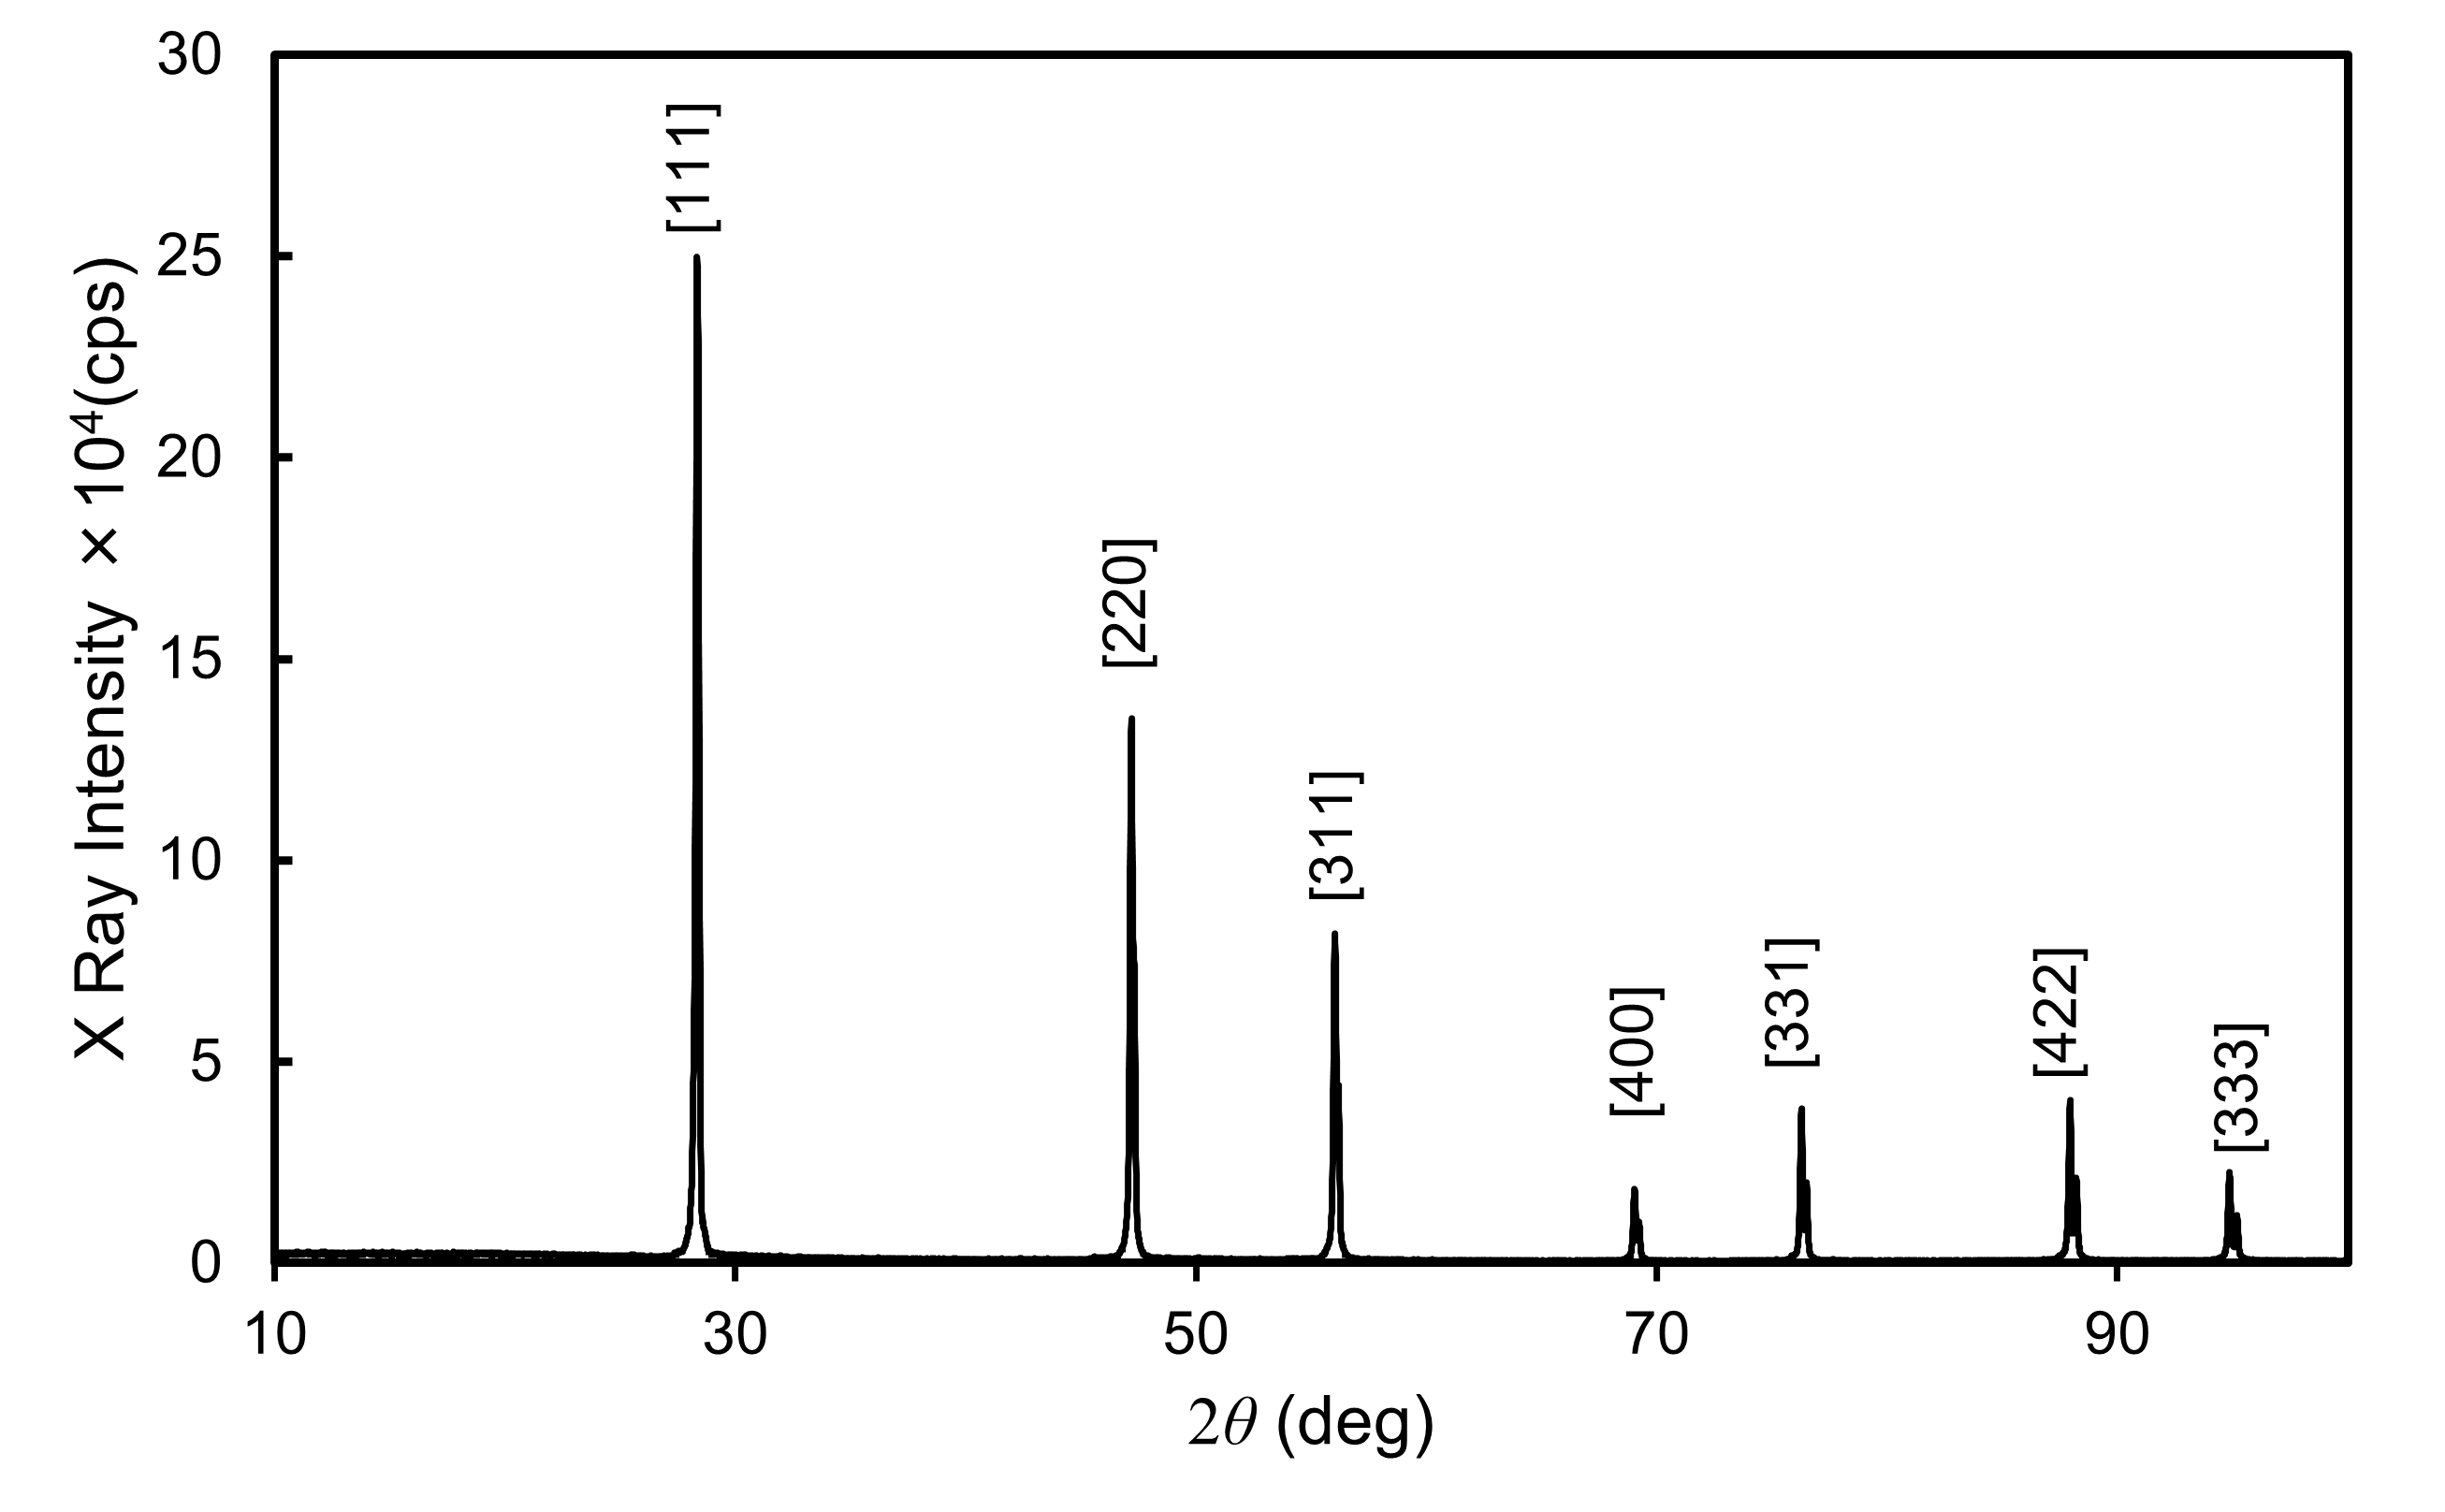
\includegraphics[width=\columnwidth]{/graph/Si.png}
		\caption{Si 単体粉末の X 線回折強度}
		\label{Si_XRD}
	\end{minipage}
	\hfil
	\begin{minipage}[t]{0.48\columnwidth}
		\centering
		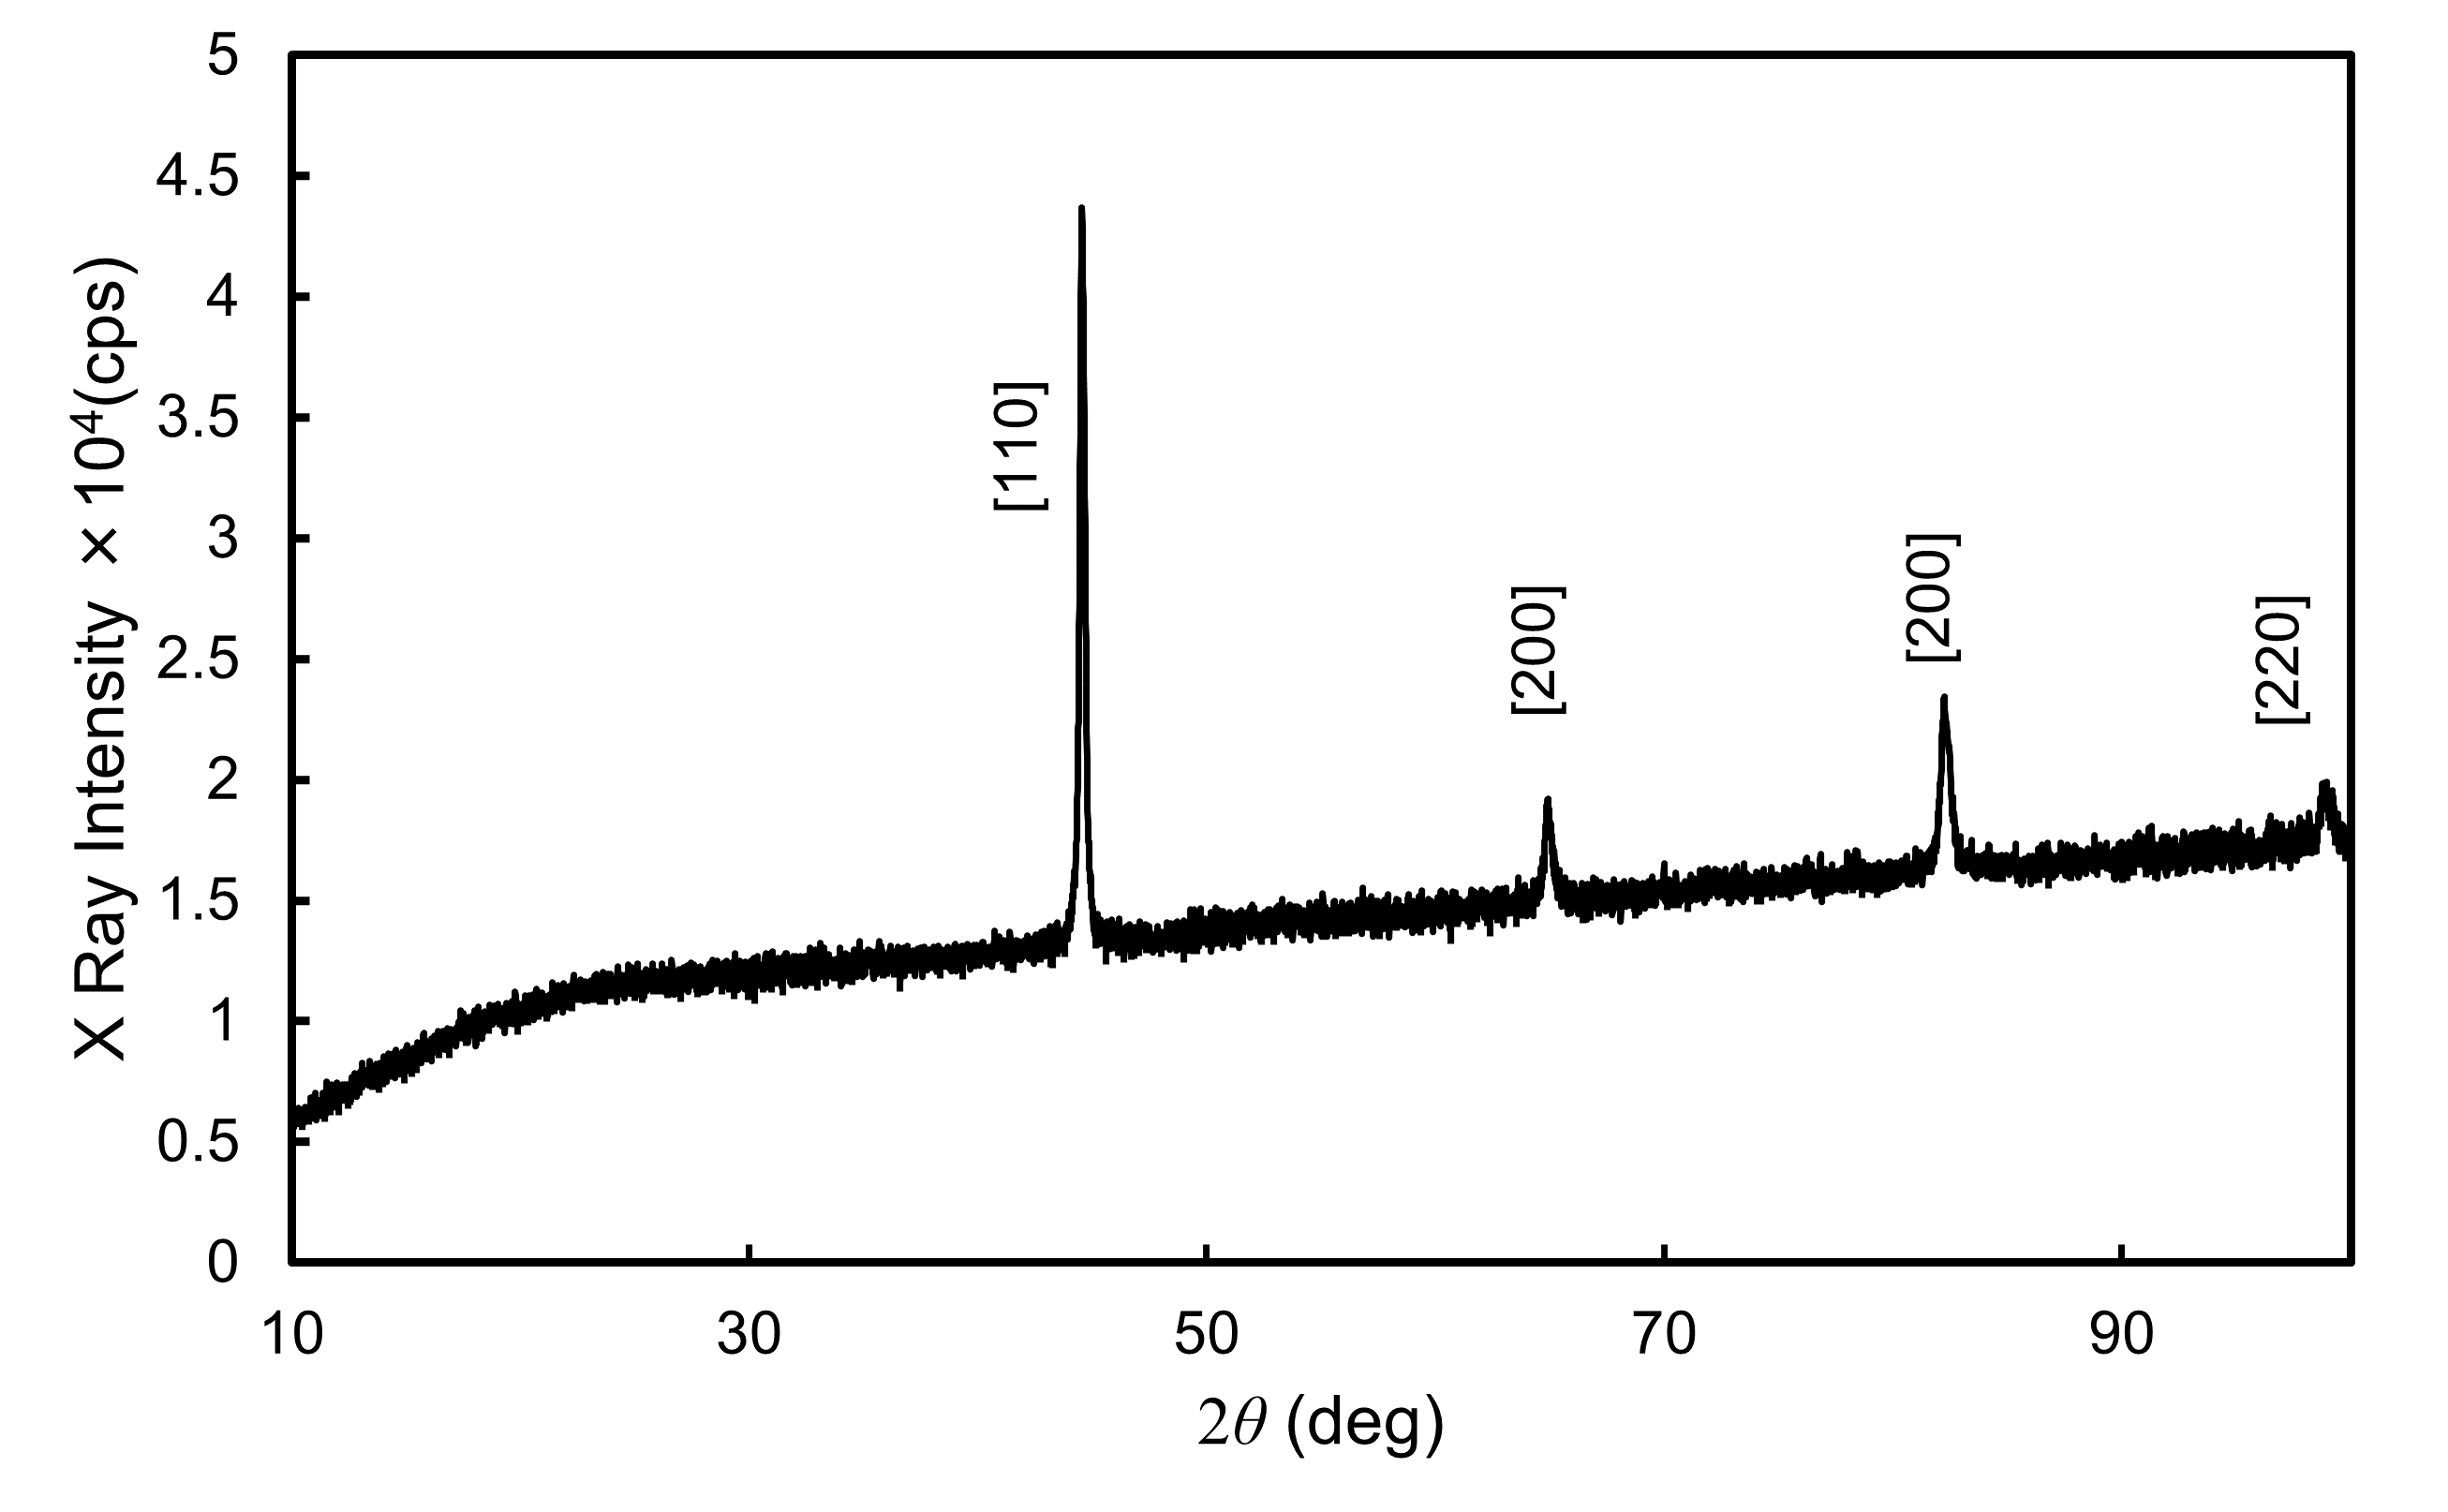
\includegraphics[width=\columnwidth]{/graph/Fe.png}
		\caption{Fe 単体粉末の X 線回折強度}
		\label{Fe_XRD}
	\end{minipage}
\end{figure}
\begin{figure}[H]
	\centering
	\begin{minipage}[t]{0.48\columnwidth}
		\centering
		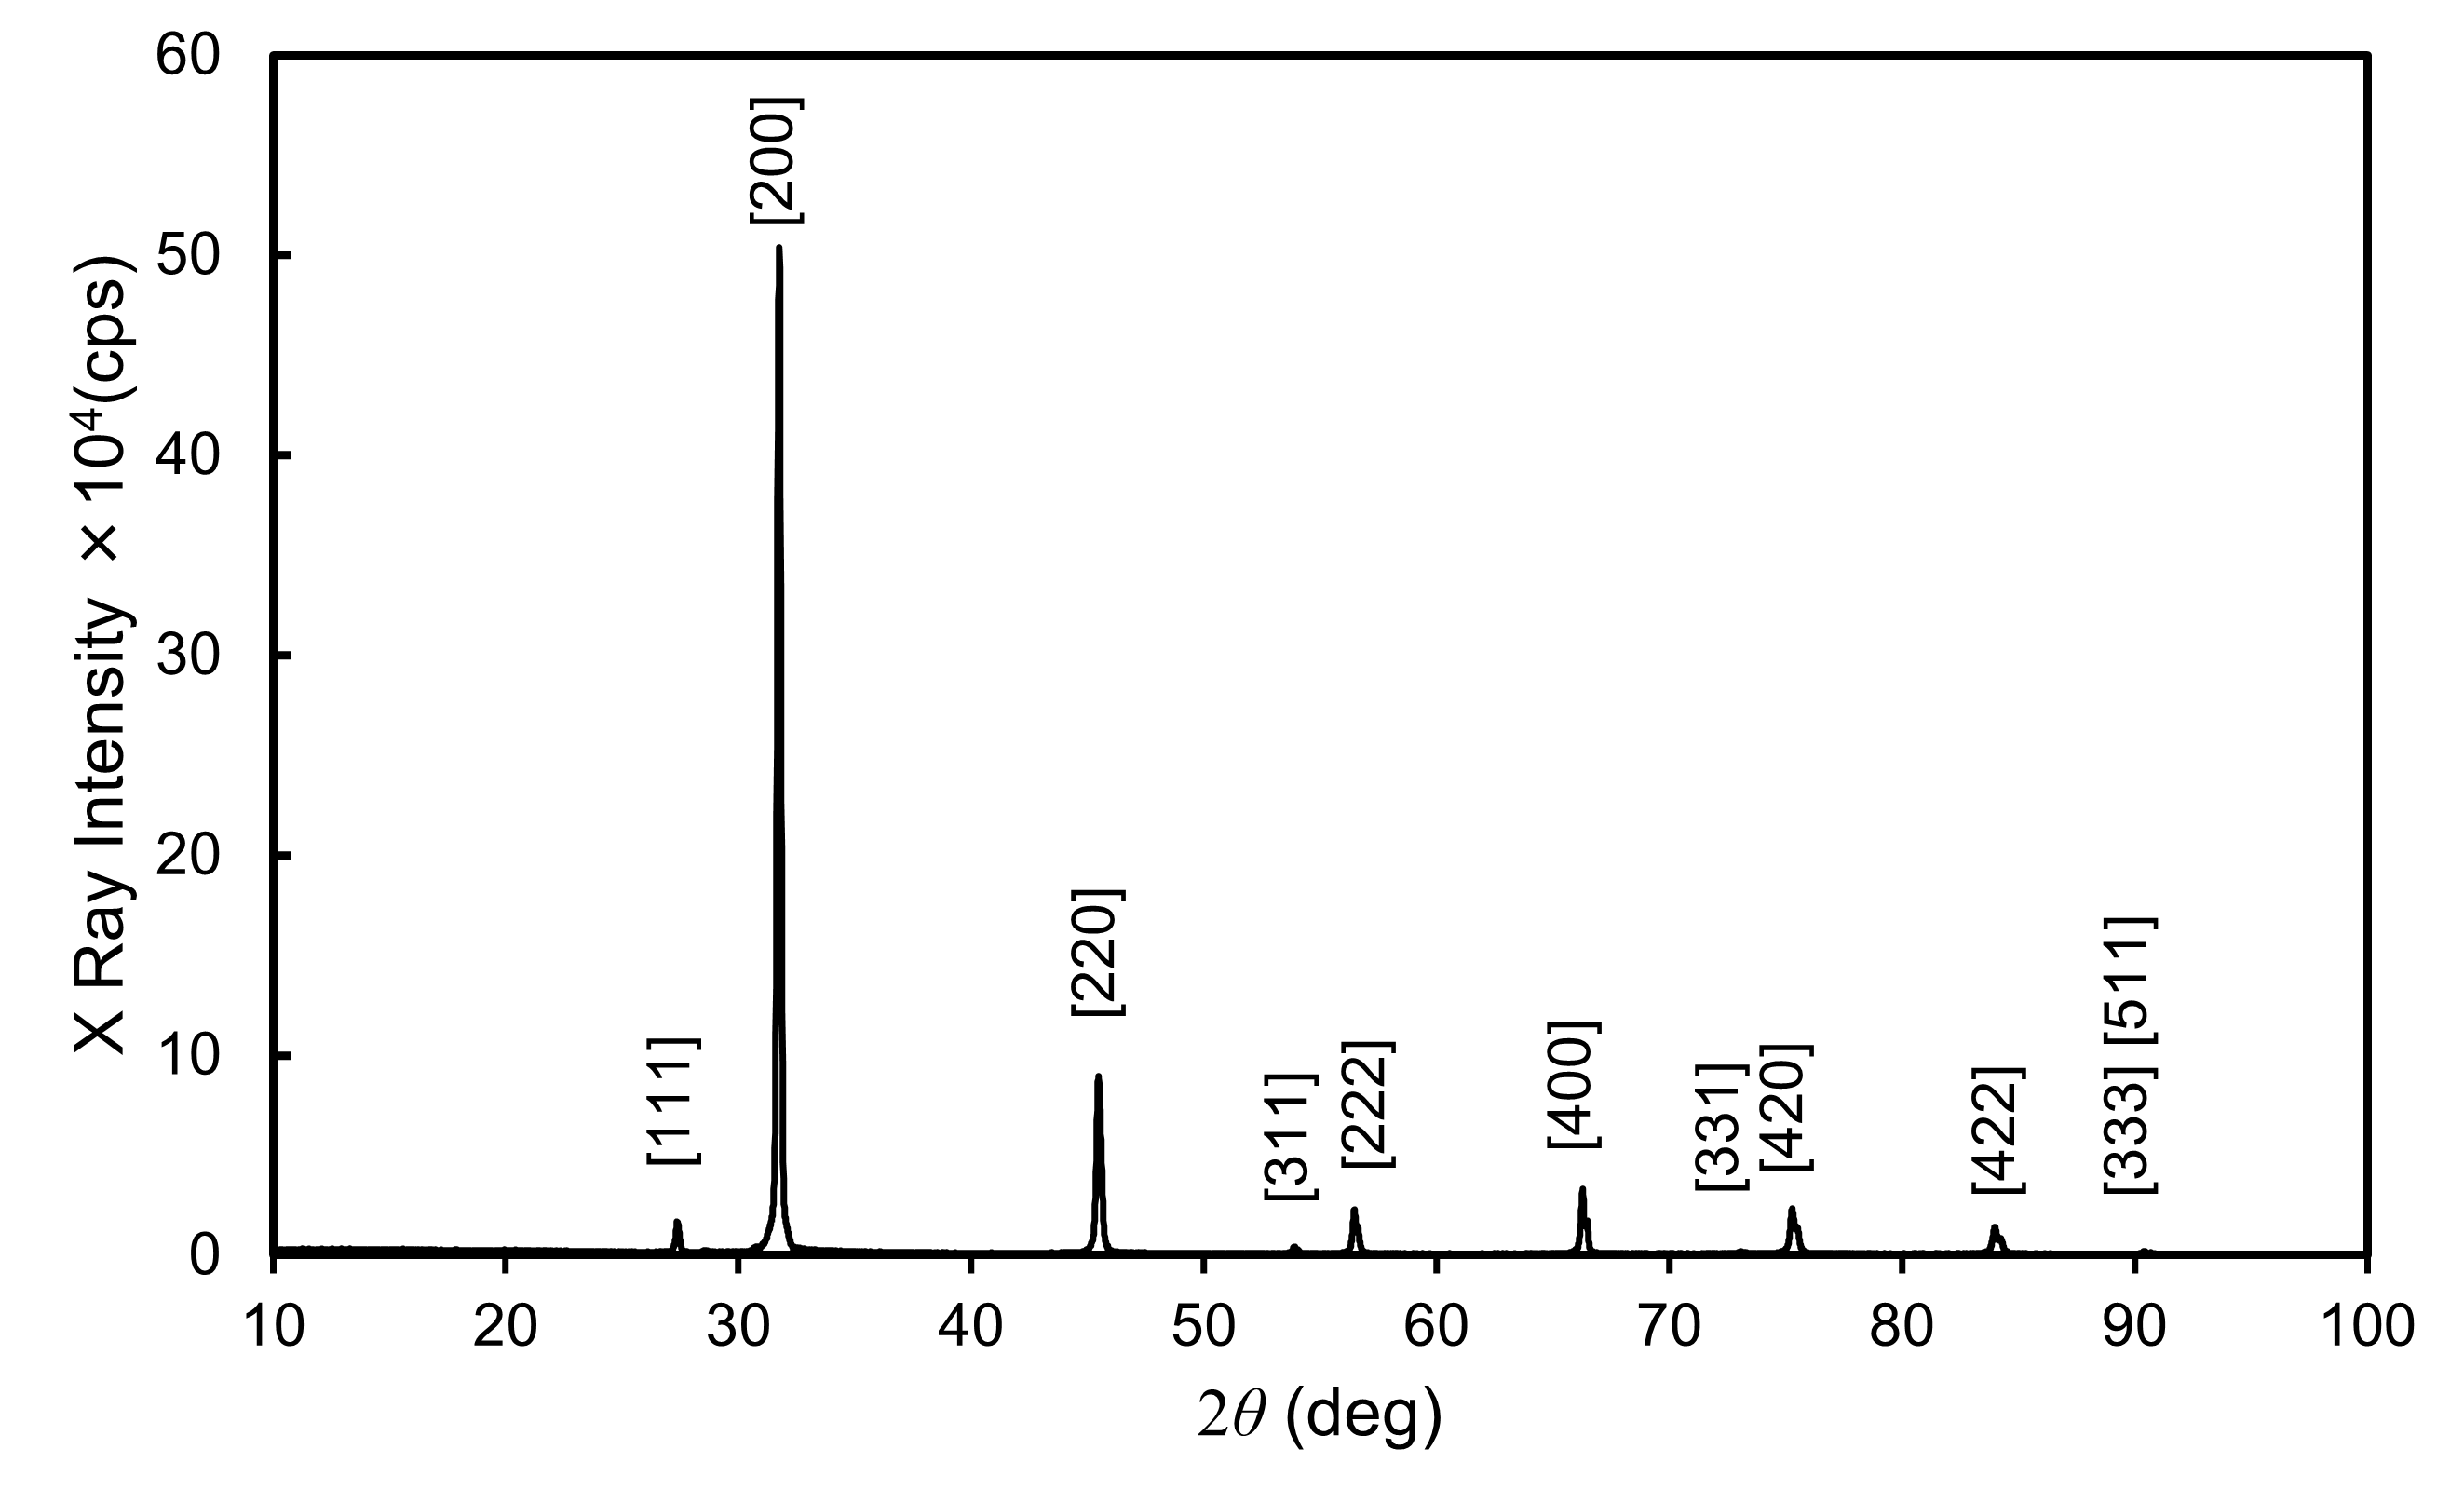
\includegraphics[width=\columnwidth]{/graph/NaCl.png}
		\caption{NaCl 粉末の X 線回折強度}
		\label{NaCl_XRD}
	\end{minipage}
	\hfil
	\begin{minipage}[t]{0.48\columnwidth}
		\centering
		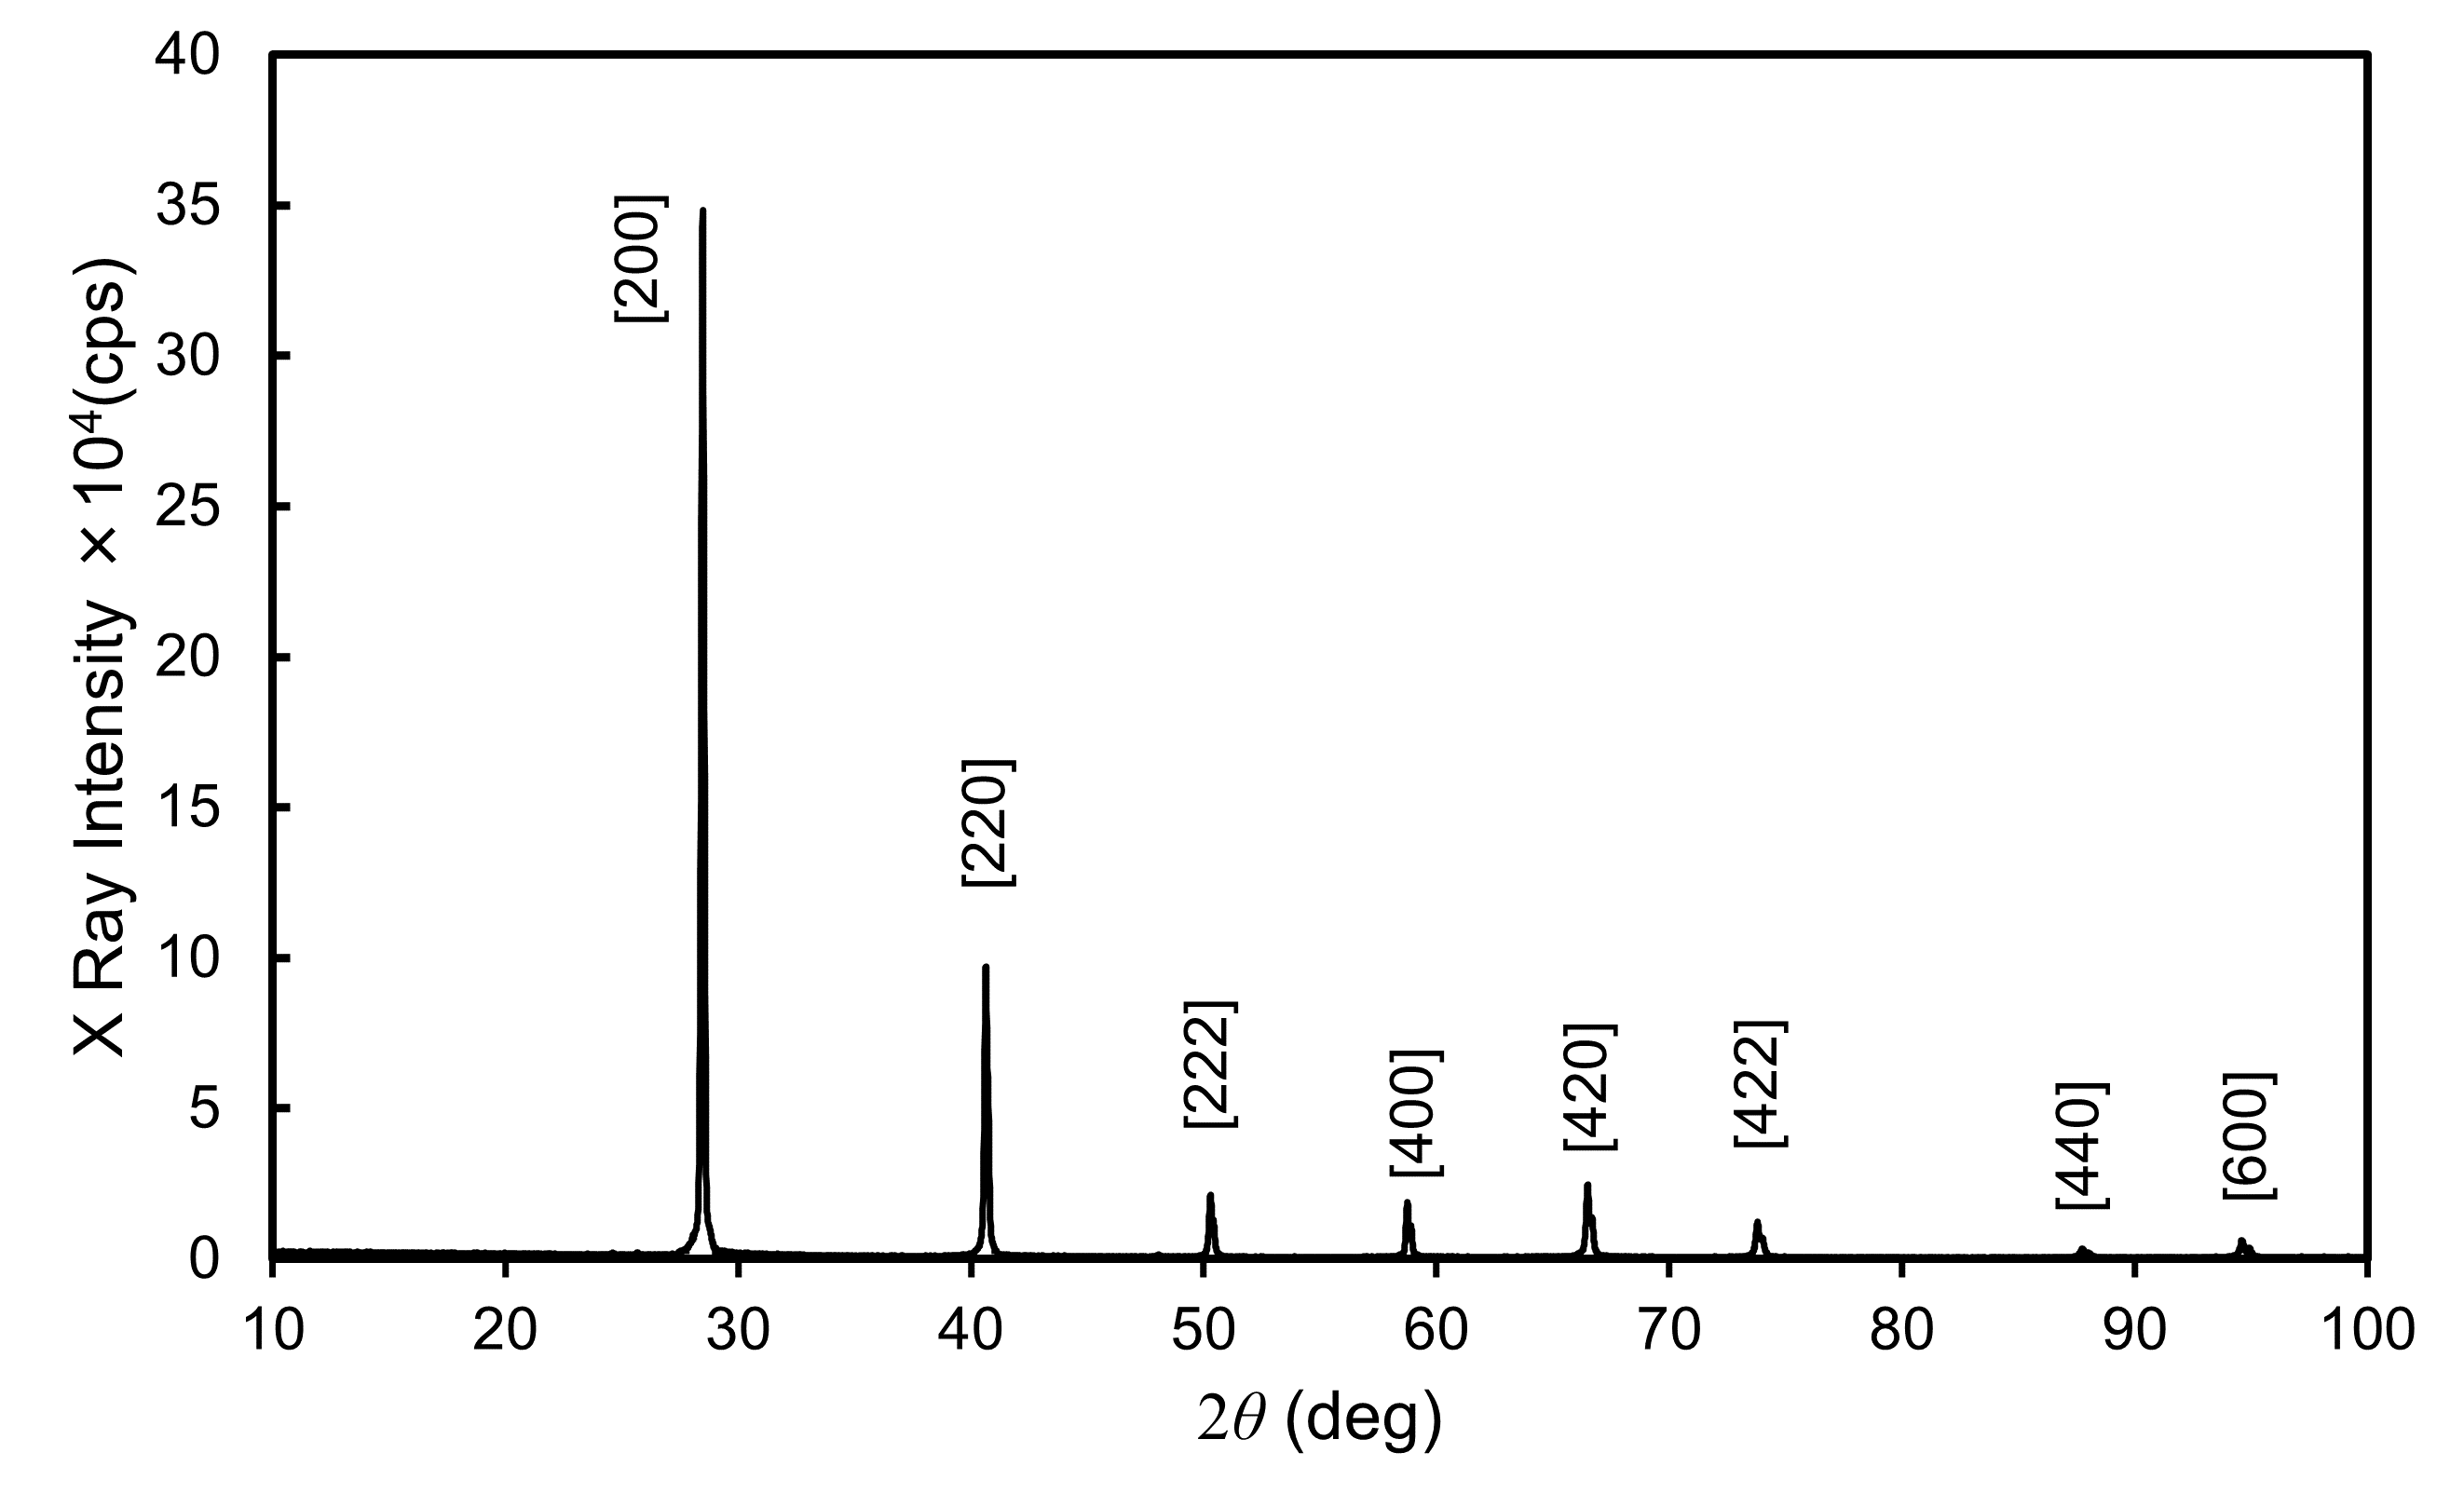
\includegraphics[width=\columnwidth]{/graph/KCl.png}
		\caption{KCl 粉末の X 線回折強度}
		\label{KCl_XRD}
	\end{minipage}
\end{figure}
\begin{figure}[H]
	\centering
	\begin{minipage}[t]{0.48\columnwidth}
		\centering
		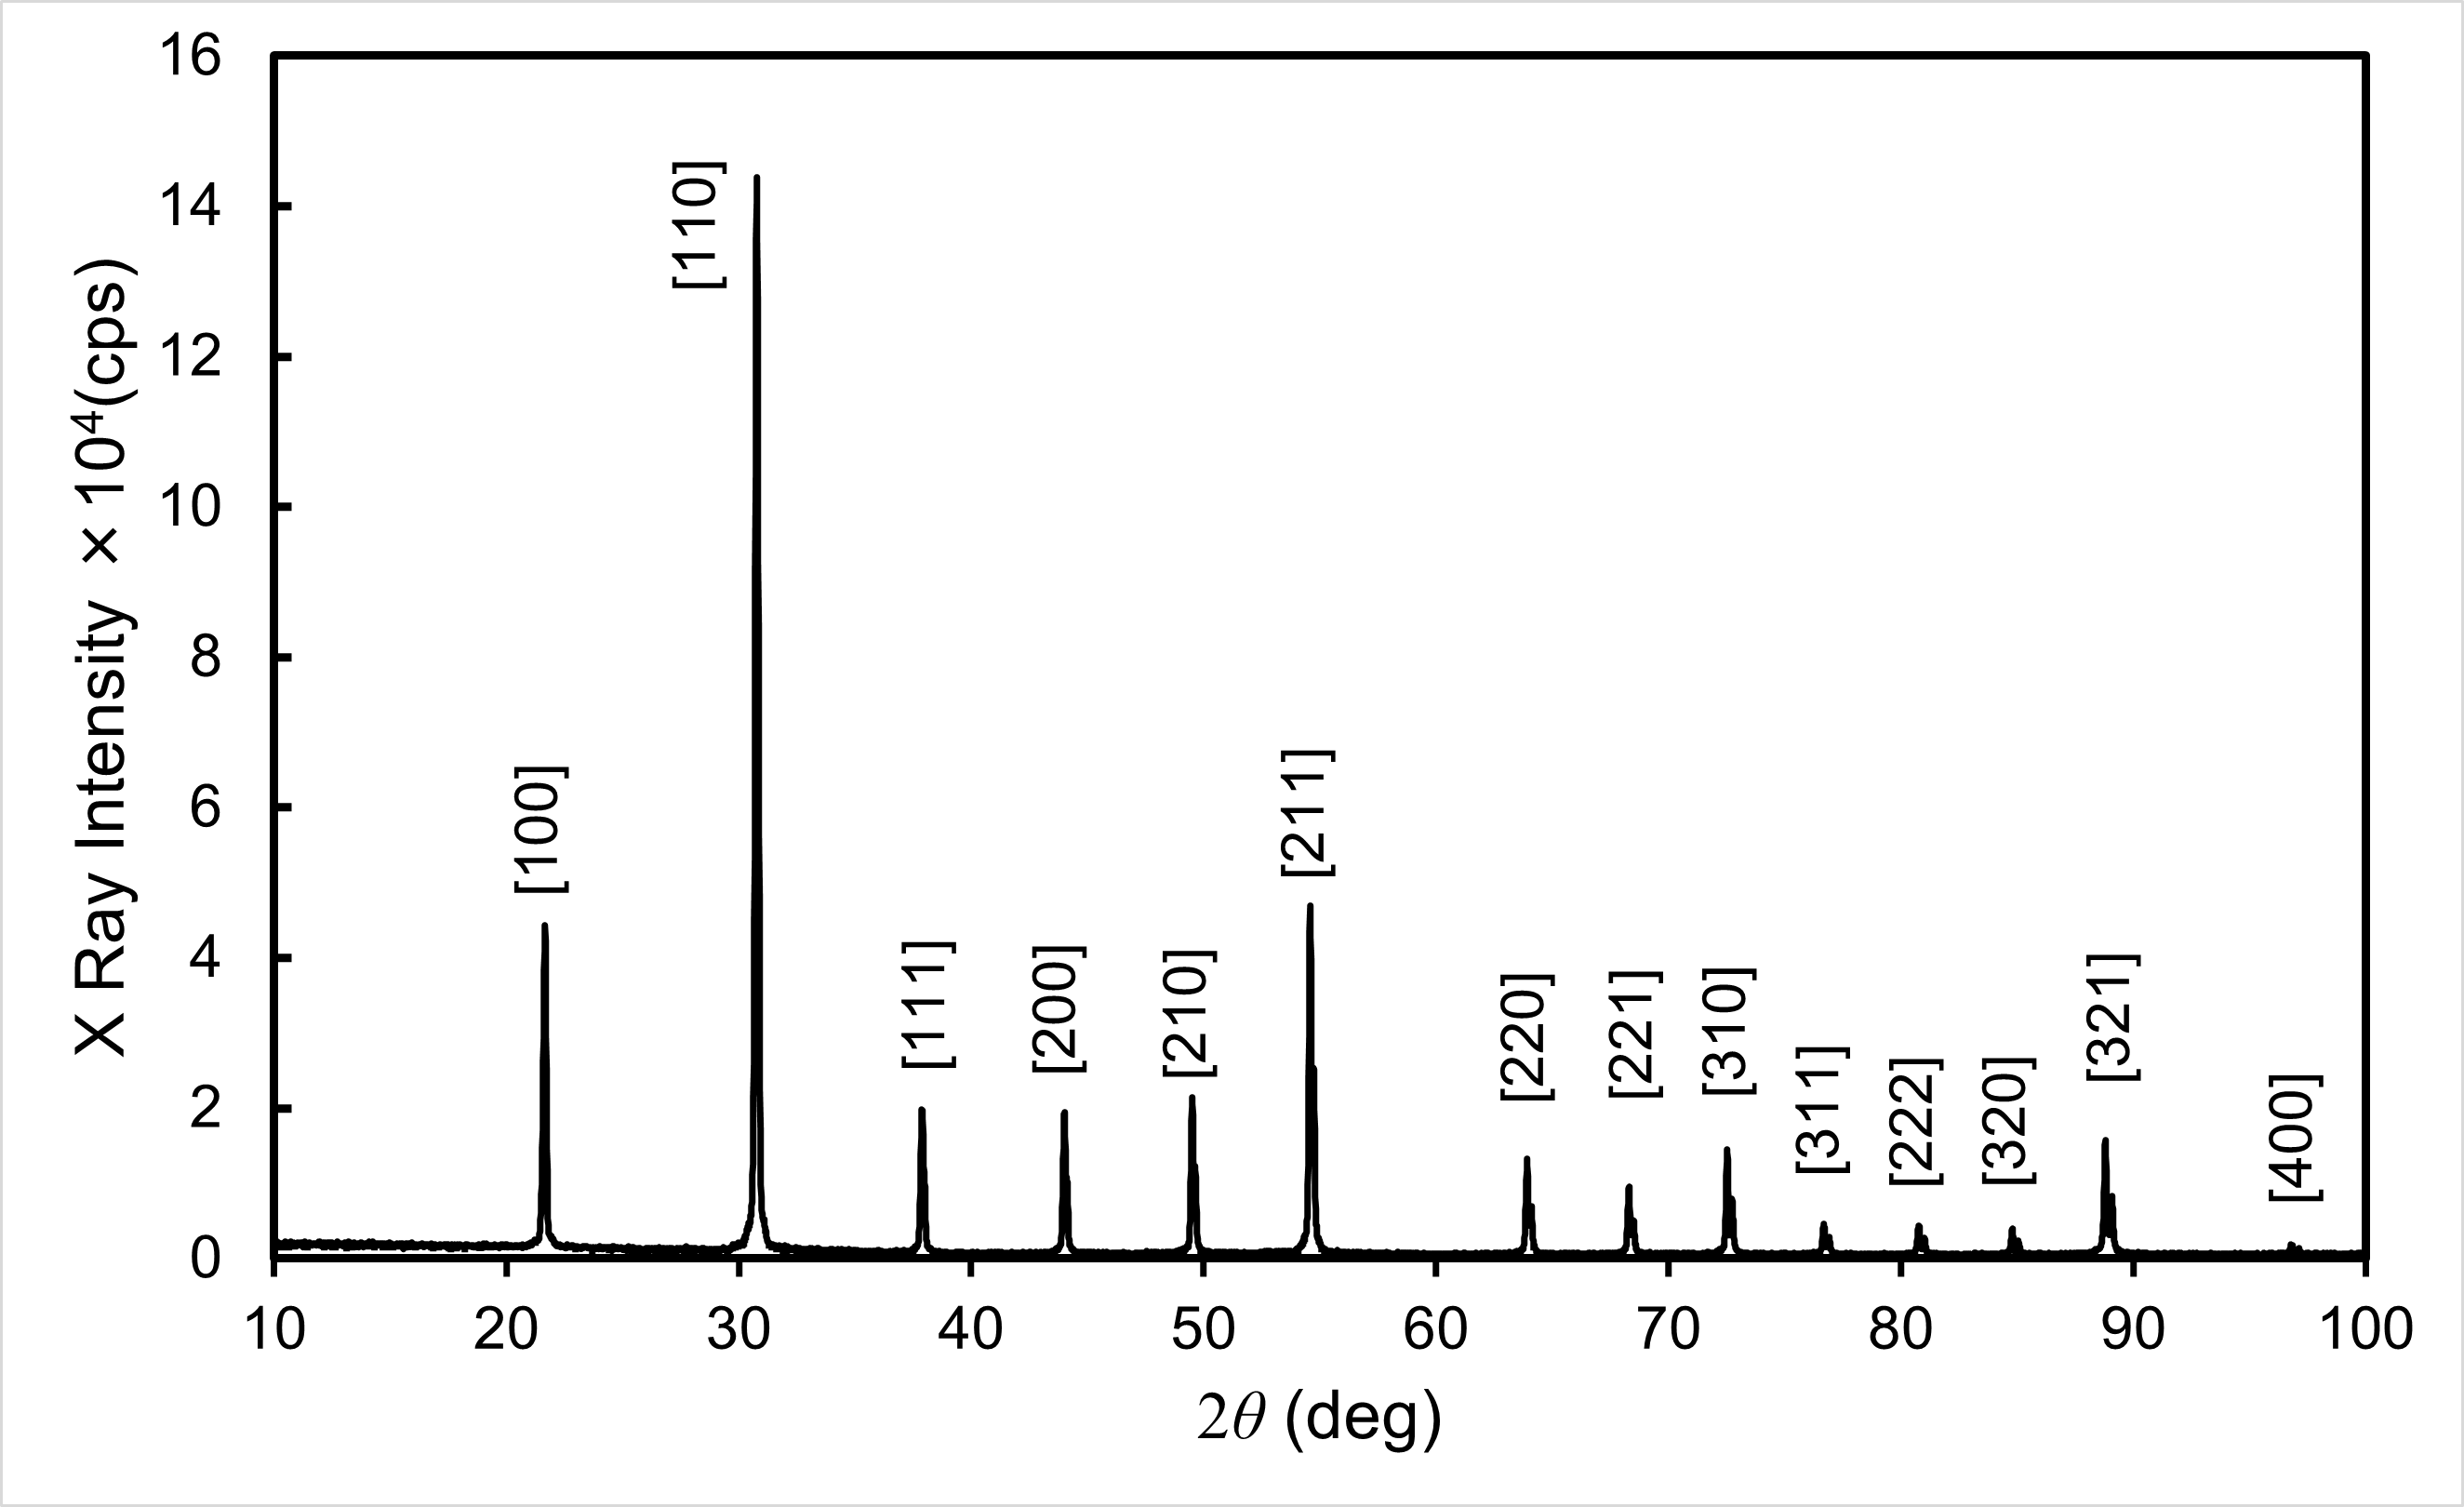
\includegraphics[width=\columnwidth]{/graph/CsCl.png}
		\caption{CsCl 粉末の X 線回折強度}
		\label{CsCl_XRD}
	\end{minipage}
\end{figure}

\section{課題}
\subsection*{課題1}
以下の 3 組の、結晶構造が同じ、あるいは似た試料の XDR 回折の結果を比較して、違いが出る理由を考察せよ。\\
(i) Fe と CsCl \quad (ii) Cu と Si \quad (iii) NaCl と KCl\\ \\

\subsubsection*{(1)}
両者とも単位格子は体心立方構造のようになっている。(図\ref{Fe_str.}, \ref{CsCl_str.})
しかし散乱強度における結晶構造因子を考えると Fe の場合
\begin{align}
	F = f_{\text{fe}}\qty(1+e^{i\pi(h+k+l)})
\end{align}
なのに対し CsCl は
\begin{align}
	F = f_{\text{Cs}}+f_{\text{Cl}}e^{i\pi(h+k+l)}
\end{align}
となる。CsCl のイオンによる散乱因子は Cs と Cl では違うので、
面指数 (hkl) の和が奇数のときであっても消滅則が働かない。
そのため XDR で検出したピークの数は CsCl のほうが多くなる。(図\ref{Fe_XRD}, 図\ref{CsCl_XRD})
Fe の強度が弱くなっているのは Fe 結晶構造というよりかはの特性によるものである。
これは考察で言及する。\\

\begin{figure}[H]
	\centering
	\begin{minipage}[t]{0.48\columnwidth}
		\centering
		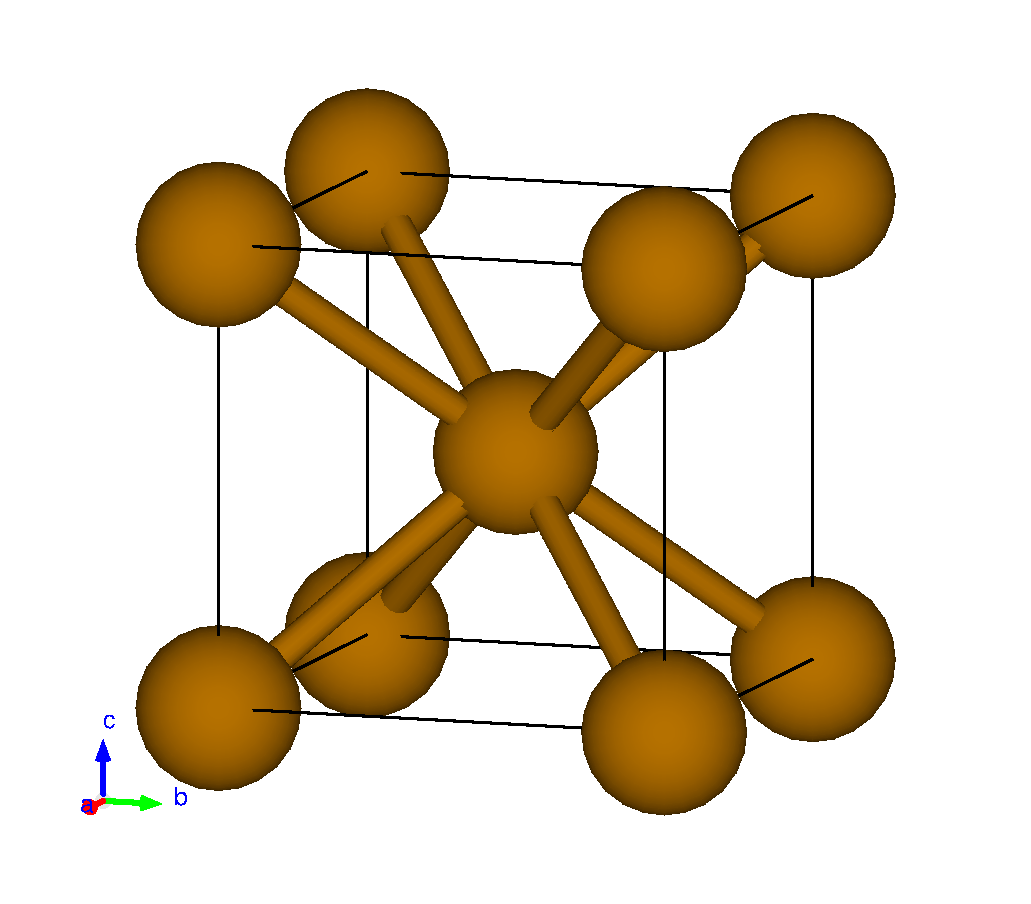
\includegraphics[width=\columnwidth]{fig/Fe.pdf}
		\caption{Fe の構造。VESTA を用いて以下の文献のパラメータを用いて作成。\cite{cfi_Fe}}
		\label{Fe_str.}
	\end{minipage}
	\hfill
	\begin{minipage}[t]{0.48\columnwidth}
		\centering
		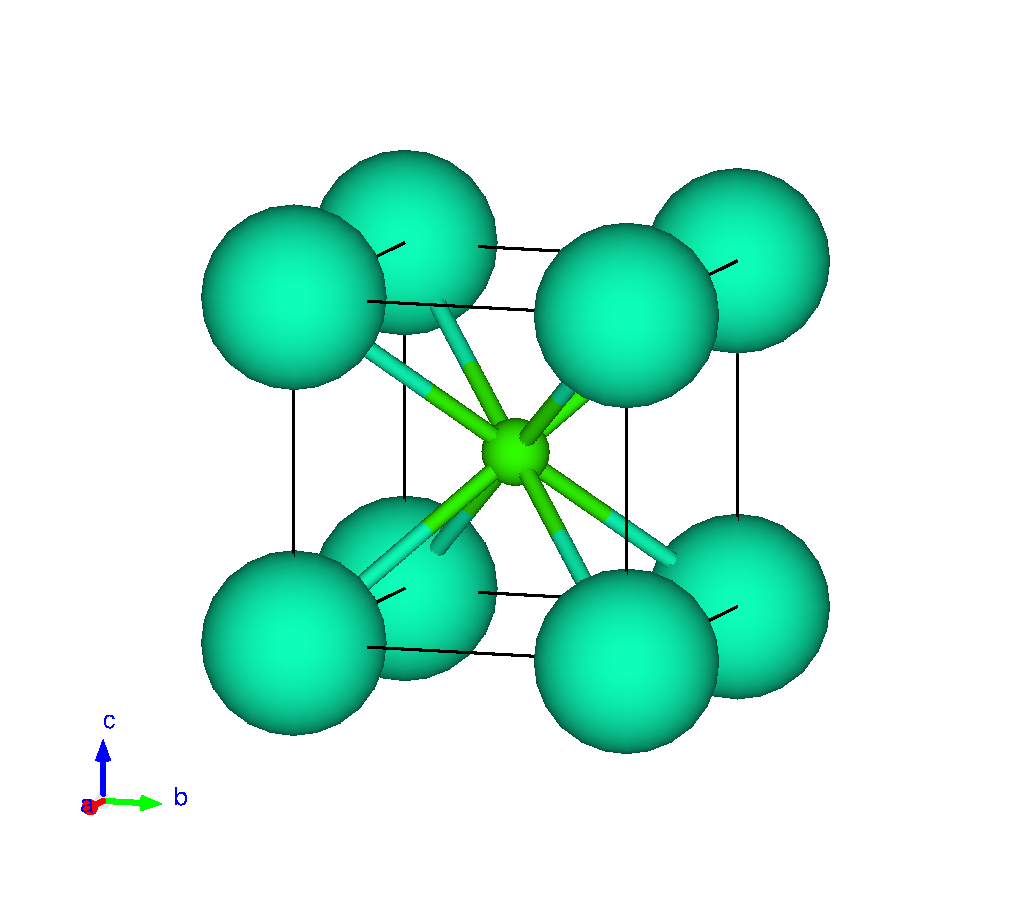
\includegraphics[width=\columnwidth]{fig/CsCl.pdf}
		\caption{Fe の構造。VESTA を用いて以下の文献のパラメータを用いて作成。\cite{cfi_CsCl}}
		\label{CsCl_str.}
	\end{minipage}
\end{figure}

\subsubsection*{(ii)}
両者とも単位格子に面心立方格子が含まれている。(図\ref{Cu_str.}, \ref{Si_str.})
Si はこれにさらに面心立方構造を(1/4, 1/4, 1/4)方向にずらした副格子もある。%副格子ってあってる?
そのため結晶構造因子は Cu のものは
\begin{align}
	F = f_{\text{Cu}}\qty(1+e^{i\pi(h+k)}+e^{i\pi(k+l)}+e^{i\pi(l+h)})
\end{align}
であり、Si は
\begin{align}
	F = f_{\text{Si}}\qty(1+e^{\frac{i\pi}{2}(h+k+l)})\qty(1+e^{i\pi(h+k)}+e^{i\pi(k+l)}+e^{i\pi(l+h)})
\end{align}
となる。
これを見ると Si の XDR のピークが消えずに残る条件は、
面心立方の消滅則である面指数 (hkl) のすべての指数の偶奇が一致しているときに加え、
(hkl) の和を4で割ったあまりが2ではないという条件が加わる。
測定できたピークの数としては Si の方が多いが面間隔のことを考えると、
やはり消滅則が多い Si は消滅しているピークがあることがわかる。(図\ref{Cu_XRD}, 図\ref{Si_XRD})% 図の参照を加えたい
Cu にはバックグラウンドが多いことは考察で言及する\\ % かもしれない
\begin{figure}[H]
	\centering
	\begin{minipage}[t]{0.48\columnwidth}
		\centering
		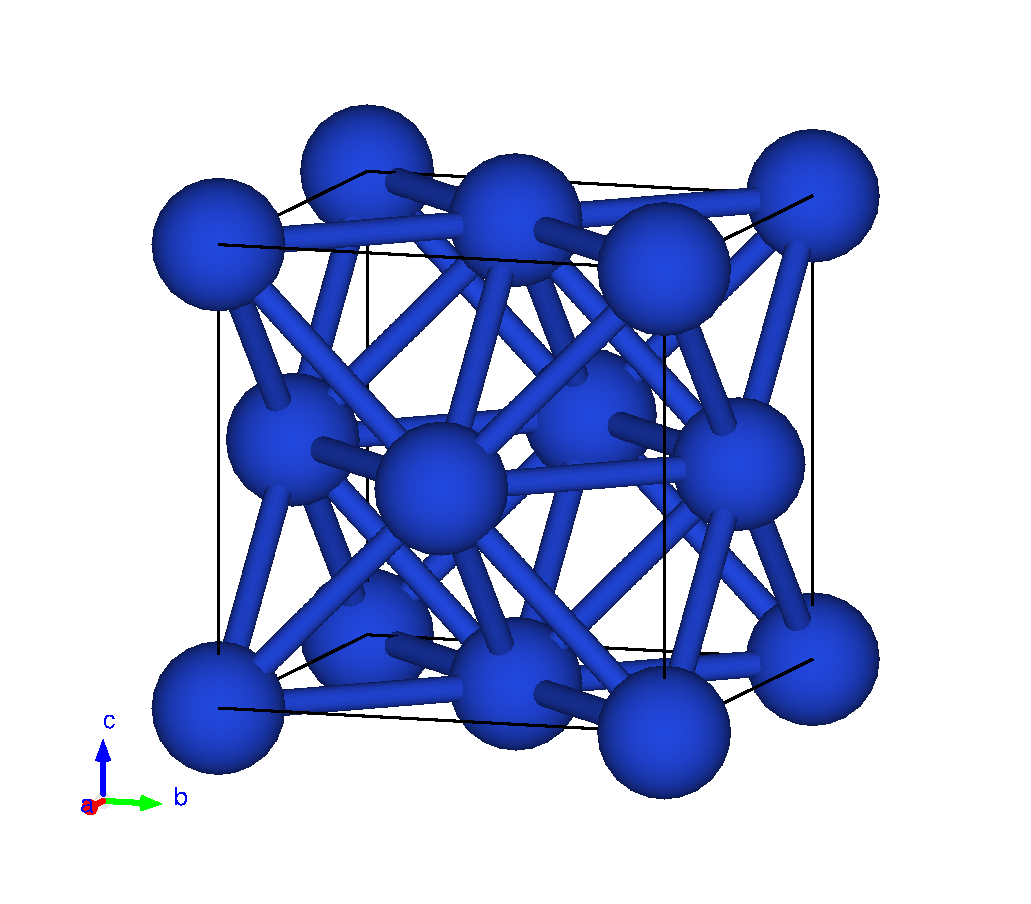
\includegraphics[width=\columnwidth]{fig/Cu.pdf}
		\caption{Cu の構造。VESTA を用いて以下の文献のパラメータを用いて作成。\cite{cfi_Cu}}
		\label{Cu_str.}
	\end{minipage}
	\hfill
	\begin{minipage}[t]{0.48\columnwidth}
		\centering
		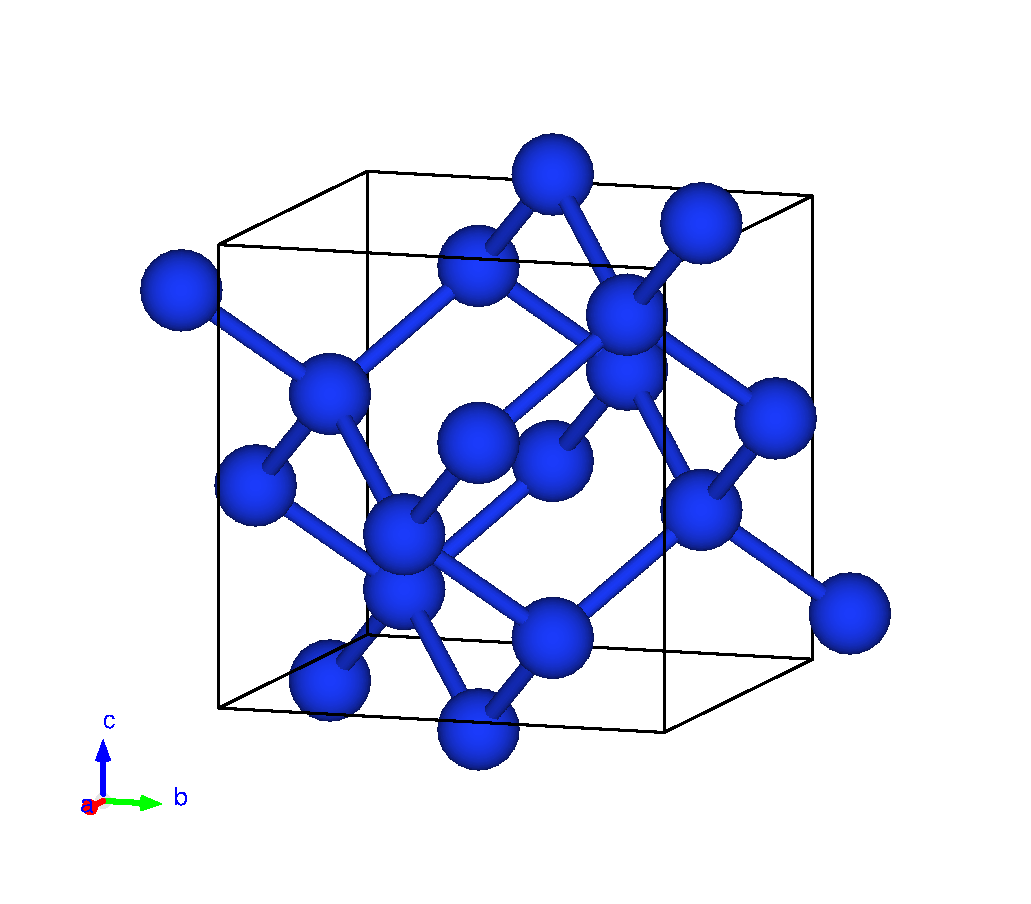
\includegraphics[width=\columnwidth]{fig/Si.pdf}
		\caption{Si の構造。VESTA を用いて以下の文献のパラメータを用いて作成。\cite{cfi_Si}}
		\label{Si_str.}
	\end{minipage}
\end{figure}

\subsubsection*{(iii)}
両者とも結晶構造としては同じ構造である。(図\ref{NaCl_str.}, \ref{KCl_str.})
しかし両者を比較すると KCl では消滅しているピークがある。(図\ref{NaCl_XRD}, 図\ref{KCl_XRD})
これは X 線の回折に関わるイオンの散乱因子の違いからくるであると考えられる。
イオンの散乱因子は希ガス核と同じだと考えると、
Na は Ne 核、Cl と K は Ar 核になるので結晶構造因子は
NaCl では
\begin{align}
	F = \qty(f_{\text{Ne}}+f_{\text{Ar}}e^{i\pi h})\qty(1+e^{i\pi(h+k)}+e^{i\pi(k+l)}+e^{i\pi(l+h)})
\end{align}
となり、KCl では
\begin{align}
	F = f_{\text{Ar}}\qty(1 + e^{i\pi h})\qty(1+e^{i\pi(h+k)}+e^{i\pi(k+l)}+e^{i\pi(l+h)})
\end{align}
となる。
これより面指数 h が奇数か偶数かという消滅則が KCl には働く。
\begin{figure}[H]
	\centering
	\begin{minipage}[t]{0.48\columnwidth}
		\centering
		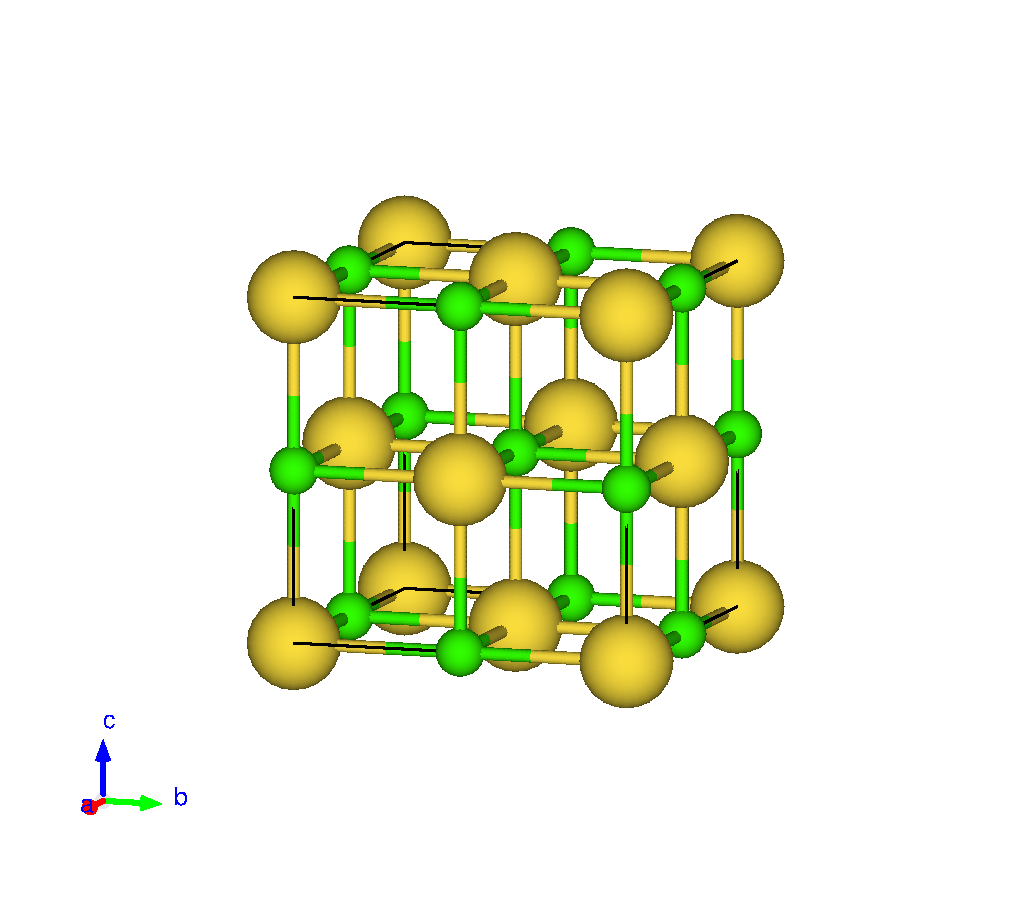
\includegraphics[width=\columnwidth]{fig/NaCl.pdf}
		\caption{NaCl の構造。VESTA を用いて以下の文献のパラメータを用いて作成。\cite{cfi_NaCl}}
		\label{NaCl_str.}
	\end{minipage}
	\hfill
	\begin{minipage}[t]{0.48\columnwidth}
		\centering
		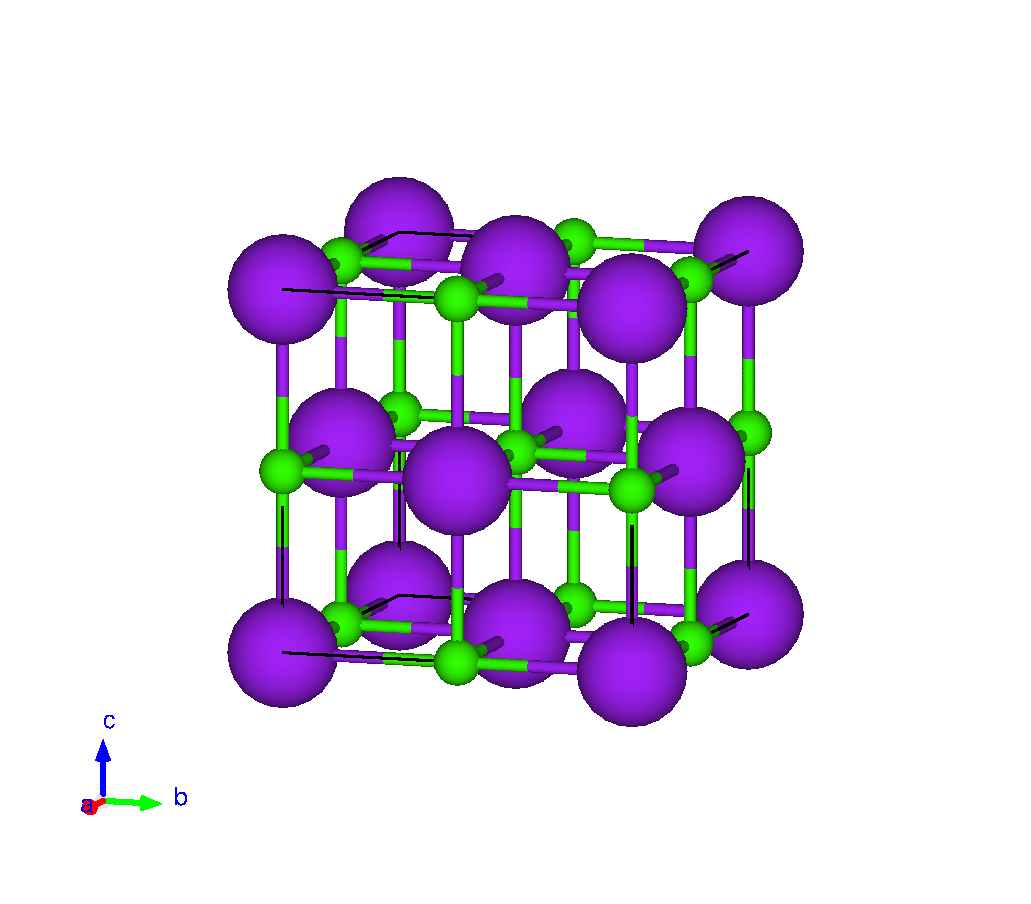
\includegraphics[width=\columnwidth]{fig/KCl.pdf}
		\caption{KCl の構造。VESTA を用いて以下の文献のパラメータを用いて作成。\cite{cfi_NaCl}}
		\label{KCl_str.}
	\end{minipage}
\end{figure}

\subsection*{課題2} 仮にこれらの立方晶の物質が、
何らかの摂動を受けて正方晶になったとする。
このとき、X 線回折パターンにはどのような変化が起こるかを推測せよ。
そして測定した物質の中から1つを例にとり、この推測に沿って具体的に議論せよ。\\

定性的には\{111\} 面のような等方的な面によるピークは変わらず、
\{220\} 面のような面指数が異なる面によるピークは 1:2 の強度比で分裂するであろうと考えられる。

\{111\} 面はどの指数を c 軸に取ったとしてもその面の形状は変わらない。% 図を描きたい
しかし \{220\} のときは指数が2の方向を c 軸に取るのと、面指数が0の方向を c 軸に取るのとでは面の形状は変わる。
c 軸の取り方は面指数が 2 の方向を取るのは 2 通り、 0 の方向を取るのは 1 通りであるため、
粉末にしたとき面の向く割合が 1:2 になるため強度のピークは変わる。

まとめると c 軸だけ伸びたとき \{hkl\} 面が分裂するかどうかによる。

\subsection*{課題3}
Cu の粉末 X 線回折結果の強度比 \(I^{\text{obs.}}\)と
付録に説明してある式 (S1)を利用して計算した強度比 \(I^{\text{cal.}}\)
を比較し、議論せよ。
ここで強度比は、最も強い回折ピークの強度を 100 として答えよ。

時間が足らず割愛します。

\section{考察}
\subsection{Fe の X 線回折強度について}
図\ref{Fe_XRD} を見るとバックグラウンドが大きくまた、回折強度も弱い。
これは X 線源から K\(\beta\) 線を取り除くのに使った Ni と Fe が似た構造をしているからであるからと考えられる。
Ni は [Ar]3d\(^8\)4s\(^2\) なのに対し、Fe は [Ar]3d\(^6\)4s\(^2\) である。
そのため電子が空軌道に遷移して光子を吸収する波長というのが近くなる。
実際理科年表\cite{rikanenpyo} の数字を参照すると Fe の K 吸収端の波長は
\begin{align}
	\lambda = 1.743 \,\text{\AA}
\end{align}
である。そのためどの Cu の特性 X 線も吸収してしまう。

K系の特性 X は 1s 電子が励起して 2p 軌道や 3p 軌道からもとに戻るときに放出される光子を使っている。
これはつまり線源の原子において 1s 軌道から 2p 軌道への励起に必要なエネルギーを特性 X 線は持つことになる。
原子番号が大きくなるにつれて 1s 軌道と 2p 軌道とのエネルギー差が大きくなるので、
線源より小さい原子番号をもつようなターゲット試料では特性 X 線の持つエネルギーが空の軌道へと励起できるような量となる。

以上より、ターゲット試料が X 線を吸収しないような線源の選び方として、
ターゲット試料の原子番号より十分大きいものを選ぶべきと考えられる。

\subsection{イオン結晶の発光}
イオン結晶の X 線回折パターンを測定したあと、装置から出すと発光していることを確認した。(図\ref{photo:ion})
\begin{figure}[H]
	\begin{minipage}[t]{0.3\columnwidth}
		\centering
		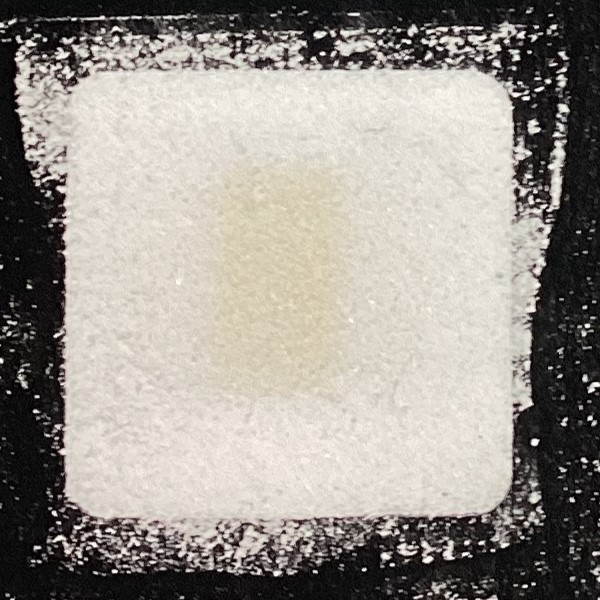
\includegraphics[width=\columnwidth]{/photo/IMG_0215.JPG}
		\subcaption{NaClが黄色に発光している。}
	\end{minipage}
	\hfill
	\begin{minipage}[t]{0.3\columnwidth}
		\centering
		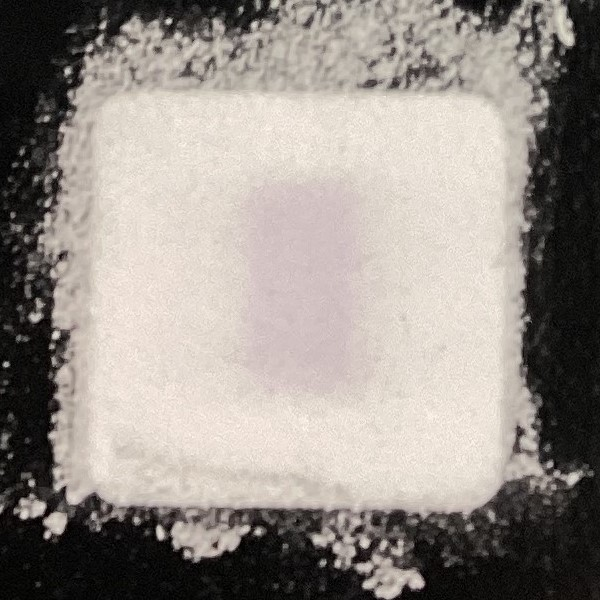
\includegraphics[width=\columnwidth]{/photo/IMG_0216.JPG}
		\subcaption{KClが紫色に発光している。}
	\end{minipage}
	\hfill
	\begin{minipage}[t]{0.3\columnwidth}
		\centering
		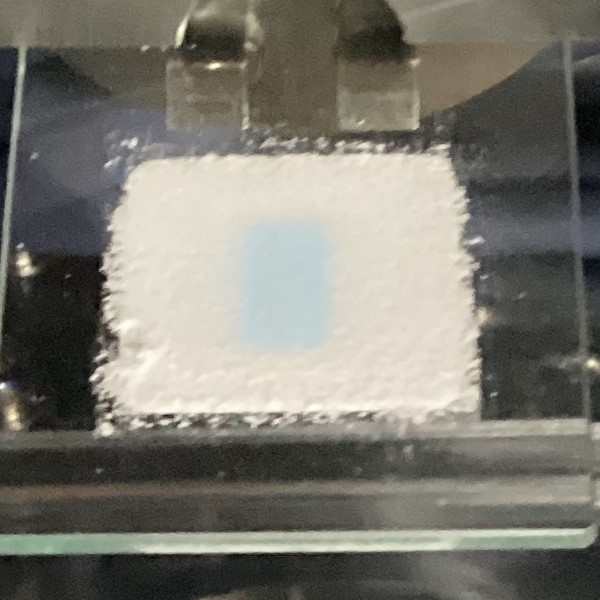
\includegraphics[width=\columnwidth]{/photo/IMG_0218.JPG}
		\subcaption{CsClが青色に発光している。}
	\end{minipage}
	\caption{X 線を照射した後のイオン結晶の様子}
	\label{photo:ion}
\end{figure}


\section{結論}
X 線材料 Cu, Si, Fe の単体粉末と、NaCl, KCl, CsCl の
粉末試料にCu の特性 X 線を入射したときの回折パターンから測定系の系統誤差を取り除いてその試料の格子定数をもとめることができた。

またこの測定において Fe は線源の X 線を吸収するため回折パターンの SN 比が悪くなることから、
別の系で測定した方がよいとわかった。

NaCl, KCl, CsCl に X 線を当てるとルミネッセンスを生じることを確認した。

\bibliographystyle{junsrt}
\bibliography{reference}

\end{document}